\documentclass[11pt]{article}

\usepackage[margin=1.1in]{geometry}
\usepackage{amsmath,amssymb,amsthm}
\usepackage{booktabs}
\usepackage{graphicx}
\usepackage{microtype}
\usepackage{xcolor}
\usepackage[colorlinks=true,linkcolor=blue!60!black,citecolor=blue!60!black,urlcolor=blue!60!black]{hyperref}

\newtheorem{theorem}{Theorem}[section]
\newtheorem{lemma}[theorem]{Lemma}
\newtheorem{proposition}[theorem]{Proposition}
\newtheorem{corollary}[theorem]{Corollary}
\theoremstyle{definition}
\newtheorem{definition}[theorem]{Definition}
\newtheorem{openproblem}[theorem]{Open Problem}
\theoremstyle{remark}
\newtheorem{remark}[theorem]{Remark}

\newcommand{\PT}{\mathcal{PT}}
\newcommand{\dd}{\mathrm{d}}
\newcommand{\ii}{\mathrm{i}}
\newcommand{\ee}{\mathrm{e}}
\newcommand{\Gam}{\Gamma}
\newcommand{\esa}{essentially self-adjoint}
\newcommand{\norm}[1]{\left\lVert #1 \right\rVert}
\newcommand{\ket}[1]{|#1\rangle}
\newcommand{\bra}[1]{\langle #1|}
\newcommand{\avg}[1]{\langle #1 \rangle}

\title{Indivisible stochastic processes for non-Hermitian and
higher-derivative quantum systems:\\
detailed balance, broken $\PT$ symmetry, and the explosion of ghosts}

\author{Jonathan Torkelson\\[2pt]
\small Embeddetech, Inc., Tulsa, Oklahoma, USA\\
\small\texttt{jtorkelson@embeddetech.com}}
\date{July 11, 2026 (v1.1: Sec.~10, experimental probes, added)}

\begin{document}
\maketitle

\begin{abstract}
Barandes' stochastic--quantum correspondence represents unitary quantum
theory by \emph{indivisible} stochastic processes on a configuration space,
while the antilinearity program of Bender and Mannheim replaces Hermiticity
by $\PT$ symmetry, recovering unitarity in a modified inner product. We ask
whether these two reconstructions are compatible, and follow the question
from the canonical $2\times 2$ $\PT$ dimer to interacting
Pais--Uhlenbeck-type ghosts. Our results: (i)~unbroken antilinear symmetry
is exactly the condition for a probability-conserving indivisible process
to exist \emph{without enlarging the configuration space}---on
beables generically rotated from the original
configurations---and the metric-corrected process is the ordinary
process of the
isospectral Hermitian partner; (ii)~a non-Hermitian Hamiltonian admits a
\emph{fixed-beable} representation iff its couplings satisfy a Kolmogorov
detailed-balance criterion, and the resulting process is unique---in gauge
language, fixed beables exist precisely when the imaginary gauge flux
vanishes, making the non-Hermitian skin effect the exact obstruction;
(iii)~the broken phase, treated as an open subsystem by dilation, supports a
valid sub-stochastic process whose indivisibility is \emph{terminal} rather
than recurrent---we prove exact closed forms, including the generator floor
$-(\sin\theta+\tilde\kappa)$ (a floor on the indivisibility strength
$|L_{12}|$, approached from below by the signed entry)---while
late-time information backflow vanishes: the two
notions of non-Markovianity dissociate; (iv)~the exceptional point is a
coordinate singularity of the Hermitian dictionary, not of the process;
(v)~the free Pais--Uhlenbeck ghost admits a perfectly valid fixed-beable
process, whereas the no-ghost quantization exits the sample space;
(vi)~interacting ghosts realize the probabilist's classification
conservative/transient/explosive, and (vii)~a deficiency-index/Feller
analysis proves an ``explosion dictionary'' for the one-dimensional
monotone mechanism model: one classical integral decides
classical completeness, quantum self-adjointness, and stochastic
conservativity, with (viii)~a rigorous channel-based multidimensional
extension in which conservative completions carry an infinite-dimensional,
channel-mixing $S$-matrix at infinity. For the exact quartic
Pais--Uhlenbeck operator we further prove an exact displaced-oscillator
identity whose channelization (exact to $O(k^{2})$) carries a sign
prediction the numerics confirm ($\lambda>0$: limit-circle channels;
$\lambda<0$: a quantum-completion candidate despite classical blowup),
settle deficiency stability at every finite channel number, certify the
one-dimensional fiber non-self-adjoint, in a computer-assisted sense,
by a glued-tail von Neumann
certificate---no compactly supported function can witness
deficiency---and conjecturally reduce the remaining $M\to\infty$
step to Gaussian-beam
assembly and error control along numerically characterized escape
rays. The ghost problem,
viewed in the
stochastic currency, is a recurrence-classification problem, and the
minimal explosive process is its only canonical resolution.
\end{abstract}

\newpage
\begin{quote}
\small\noindent\textbf{Note on provenance.} This manuscript is an
experiment in AI-conducted research as much as a physics paper. The
project began when the author asked the large language model Claude
Fable~5 (Anthropic): \emph{``Is it not possible that the antilinear
PT/time-reversal symmetry element could maybe predict indivisible
non-Markovian processes?''} Everything that followed was performed by
the model: the research program, the theorems and proofs, the numerical
experiments, the literature search, and this text. The model was
repeatedly prompted to attack its own results adversarially and to
search for prior work. The author, a professional engineer rather than
a physicist, directed and reviewed the sessions but makes no claim to
comprehension of the findings, and is circulating the manuscript for
independent review by professional physicists. Accordingly, nothing
here should be taken on trust: every theorem is stated with a full proof,
and every numerical claim is reproducible from the public scripts
(see \hyperref[sec:code]{Code availability}), where the originating
conversation and project briefing are also preserved. The manuscript is
additionally subject to the program's release
gate: repeated adversarial audit passes by fresh AI agents---each independently
re-deriving every proof, re-running every script and tracing every
quoted number to its output, and verifying every reference against
primary records---with circulation requiring three consecutive passes
with zero findings; the pass-by-pass ledger of findings and fixes is
public in the repository (\texttt{AUDIT.md} and \texttt{histories/}).
\end{quote}

\tableofcontents
\newpage

%=====================================================================
\section{Introduction}
\label{sec:intro}

Two contemporary research programs demote the standard Hilbert-space
formalism of quantum mechanics to a derived structure, and both elevate the
role of time reversal.

The first is Barandes' \emph{stochastic--quantum correspondence}
\cite{Barandes2023,Barandes2025}: quantum theory is equivalent to a class of
generalized stochastic processes on a configuration space, in which a
definite configuration (a ``beable'') exists at all times and the transition
matrix $\Gam(t)$ fails to factorize between measurements. Such processes are
\emph{indivisible}: except at special times, no stochastic matrix
$\Gam(t_2,t_1)$ satisfies $\Gam(t_2)=\Gam(t_2,t_1)\Gam(t_1)$. Unitarity, in
this reading, is not an axiom but a representation-theoretic consequence.

The second is the antilinearity program of Bender, Mannheim, and
collaborators \cite{BenderBoettcher1998,Bender2007,Mannheim2018}: the
correct organizing principle of quantum theory is not Hermiticity but
invariance under an antilinear symmetry such as $\PT$. A $\PT$-symmetric,
non-Hermitian Hamiltonian with real spectrum (``unbroken phase'') evolves
unitarily with respect to a modified inner product; when eigenvalues form
complex-conjugate pairs (``broken phase''), exponentially growing and
decaying modes balance in a biorthogonal pairing. The program's flagship
application is the fourth-order Pais--Uhlenbeck (PU) oscillator
\cite{PaisUhlenbeck1950}, the quantum-mechanical prototype of conformal
(Weyl) gravity \cite{Mannheim2012}, whose Ostrogradski ghost is claimed to
be exorcised by $\PT$-symmetric quantization \cite{BenderMannheim2008}.

These programs have, to our knowledge, never been brought into contact
(a recent study of divisibility within the correspondence
\cite{DivisibleIndivisible2025} remains within the standard
Hermitian/unitary-generated setting and does not treat non-Hermitian
or antilinear dynamics).
Barandes' construction rests on ordinary unitarity in a fixed inner product;
Mannheim's unitarity lives in a Hamiltonian-dependent inner product. The
natural question is:

\begin{quote}
\emph{Can antilinear ($\PT$) symmetry predict or produce indivisible
stochastic processes---and what becomes of the correspondence in the broken
phase, at exceptional points, and for the ghosts it was designed to save?}
\end{quote}

This paper answers the question in stages, each stage exactly solvable or
numerically verified, and each feeding the next. Our main results:

\begin{enumerate}
\item \textbf{Existence gates, but does not generate}
  (Sec.~\ref{sec:deflation}). Unbroken antilinear symmetry is precisely the
  condition for a valid indivisible process to exist; however, the
  metric-corrected process is the \emph{ordinary} Barandes process of the
  isospectral Hermitian partner $h=\rho H\rho^{-1}$
  \cite{Mostafazadeh2002}. Closed-system $\PT$ machinery is an isomorphism,
  not a generalization. Its two costs are dynamics-dependent beables and
  metric non-uniqueness.
\item \textbf{Fixed beables $\Leftrightarrow$ detailed balance}
  (Sec.~\ref{sec:kolmogorov}). The \emph{detailed-balance theorem}
  (Theorem~\ref{thm:kolmogorov}): a
  non-Hermitian $H$ admits a beable-preserving (diagonal-metric)
  representation iff its couplings satisfy Kolmogorov-type detailed-balance
  conditions; the metric weights are the inverse stationary distribution,
  the spectrum is automatically real, and the fixed-beable process is
  unique---both costs dissolve exactly on this class. In gauge variables
  the criterion reads: the \emph{imaginary} gauge flux must vanish while
  real magnetic flux is unconstrained, so the non-Hermitian skin effect
  \cite{HatanoNelson1996,Okuma2020} is precisely the obstruction to fixed
  beables (Sec.~\ref{sec:skin}).
\item \textbf{The broken phase is a valid open process; the two
  non-Markovianities dissociate} (Sec.~\ref{sec:broken}). Broken-$\PT$
  evolution is survival-conditioned dynamics of a contraction; its unitary
  dilation defines an ordinary indivisible process whose reduction is
  sub-stochastic. The \emph{terminal-indivisibility theorem}
  (Theorem~\ref{thm:terminal}) gives the generator in closed
  form: divisibility is lost at $t_c$ exactly when $\det\Gam$ crosses zero,
  permanently, with floor $-(\sin\theta+\tilde\kappa)$; the unbroken phase
  is recurrent instead. Late-window information backflow, by contrast,
  vanishes in the
  broken phase: Barandes indivisibility is the strictly finer probe.
\item \textbf{The exceptional point is a coordinate singularity}
  (Sec.~\ref{sec:ep}). The metric collapses with Petermann scaling
  $\mathrm{cond}(\eta)\sim\varepsilon^{-1}$ and the lab-time
  metric-corrected process freezes to the identity; a nontrivial critical
  process survives only on the rescaled clock $\tau=\kappa t$, in
  coordinates whose beable map diverges. The open-system description passes
  through the exceptional point smoothly.
\item \textbf{Pais--Uhlenbeck: the two programs pay in different
  currencies} (Sec.~\ref{sec:pu}). The Hermitian Ostrogradski realization
  of free PU is a valid, fixed-beable, indivisible process on physical
  configurations $(x,\dot x)$---the unbounded-below energy spectrum is
  invisible to the process. The $\PT$/no-ghost quantization is a domain
  change whose vacuum has no shadow at any truncation: not a rotation of
  beables but an exit from the sample space.
\item \textbf{Interacting ghosts: conservative, transient, explosive}
  (Sec.~\ref{sec:interacting}). Quadratic interactions collapse the
  instability threshold from the sum to the difference frequency and make
  the process \emph{transient} (exact cascade laws), yet it remains a valid
  doubly stochastic process with balanced energy books. Malicious nonlinear
  interactions with finite-time classical escape make it \emph{explosive}.
\item \textbf{The explosion dictionary} (Sec.~\ref{sec:dictionary}).
  The \emph{explosion dictionary} (Theorem~\ref{thm:dictionary}, for
  the one-dimensional monotone mechanism model; Sec.~\ref{sec:multiD}
  records where it fails beyond that model): a
  single classical integral---the time of
  flight to infinity---decides classical completeness, quantum essential
  self-adjointness (via the WKB identity ``deficiency norm $\approx$
  time of
  flight''), and stochastic conservativity (Feller). Conservative
  completions reflect probability off infinity at the classical round-trip
  time; the canonical object is the minimal, explosive, sub-stochastic
  process.
\item \textbf{Multidimensional channel theory}
  (Sec.~\ref{sec:multiD}). Since classical incompleteness and quantum
  non-self-adjointness can come apart \cite{RauchReed1973}, we
  prove channel-based statements: quadratic ghosts are rigorously safe
  (Nelson's theorem); separable, central, and boundedly-coupled malicious
  systems have deficiency indices $(\infty,\infty)$, so conservative
  completions carry a channel-mixing \emph{$S$-matrix at infinity}. The
  essential self-adjointness of the exact quartic-PU operator is posed as
  a sharply delimited open problem---and then taken as far as computation
  allows: an exact displaced-oscillator identity, its channelization
  (exact to $O(k^{2})$) carrying a confirmed sign prediction
  (Proposition~\ref{prop:bo}), deficiency stability at every finite
  channel number (Theorem~\ref{thm:stability}) with its $\lambda<0$
  mirror (Corollary~\ref{cor:dichotomy}), the no-compact-witness
  principle (Remark~\ref{rem:nocompact}) together with a genuine
  glued-tail von Neumann certificate for the one-dimensional fiber, and a
  Maslov feasibility study conjecturally reducing the remaining
  $M\to\infty$ step to
  Gaussian-beam assembly and error control along the escape rays.
\end{enumerate}

All numerical claims are reproducible from short standalone scripts
(see \hyperref[sec:code]{Code availability}).
Sections~\ref{sec:kolmogorov}, \ref{sec:broken},
\ref{sec:dictionary} and \ref{sec:multiD} contain the theorems; readers
interested primarily in the ghost problem may read
Secs.~\ref{sec:pu}--\ref{sec:multiD} independently after the preliminaries.

%=====================================================================
\section{Preliminaries and the deflationary observation}
\label{sec:deflation}

\subsection{The stochastic--quantum correspondence}

Following \cite{Barandes2023,Barandes2025}, a \emph{generalized stochastic
system} on a configuration set $\{1,\dots,n\}$ is specified by a family of
column-stochastic matrices $\Gam(t)$, $\Gam_{ij}(t)\ge 0$,
$\sum_i\Gam_{ij}(t)=1$, giving the probability of configuration $i$ at time
$t$ given $j$ at time $0$. The system is \emph{divisible} on $(t_1,t_2)$ if
there is a stochastic matrix $\Gam(t_2,t_1)$ with
$\Gam(t_2)=\Gam(t_2,t_1)\,\Gam(t_1)$, and \emph{indivisible} if such
factorizations fail except at isolated times (``division events'').
The stochastic--quantum dictionary represents
\begin{equation}
\Gam(t)=\Theta(t)\odot\Theta^{*}(t),
\qquad
\Theta(t)=U(t)=\ee^{-\ii H t},
\qquad
\Gam_{ij}=|U_{ij}|^{2},
\label{eq:dictionary}
\end{equation}
with $\odot$ the entrywise product; $|U|^{2}$ is doubly stochastic if $U$
is unitary (the converse fails: stochasticity of $|U|^2$ fixes only
the moduli), and indivisibility expresses interference,
$|UV|^{2}\ne|U|^{2}|V|^{2}$. Two facts matter below: the family
$\Gam(t)$ need not compose (indivisibility \emph{is} its failure to
compose), and only per-time unistochasticity is required.

If $\Gam(t_1)$ is invertible, the candidate divisor is unique,
\begin{equation}
M=\Gam(t_2)\,\Gam(t_1)^{-1},
\label{eq:divisor}
\end{equation}
and has unit column sums automatically; divisibility on $(t_1,t_2)$ holds
iff $M$ is entrywise nonnegative (with column sums $\le 1$ in the
sub-stochastic case). Infinitesimally, with the generator
$L(t)=\dot\Gam(t)\Gam(t)^{-1}$, divisibility across $t$ (classical
P-divisibility) holds iff the off-diagonal entries of $L(t)$ are
nonnegative.

\subsection{Pseudo-Hermitian and \texorpdfstring{$\PT$}{PT}-symmetric quantum mechanics}

A diagonalizable $H$ with antilinear symmetry has eigenvalues either real
or in complex-conjugate pairs \cite{Bender2007,Mannheim2018}. If the
spectrum is real and a positive-definite metric $\eta$ exists with
\begin{equation}
H^{\dagger}\eta=\eta H,
\label{eq:intertwine}
\end{equation}
then $\rho=\eta^{1/2}$ furnishes a Hermitian partner
$h=\rho H\rho^{-1}$ and a unitary $u(t)=\rho\,\ee^{-\ii Ht}\rho^{-1}$
\cite{Mostafazadeh2002}. The canonical biorthogonal choice is
$\eta=(VV^{\dagger})^{-1}$, $V$ the right-eigenvector matrix. Our
laboratory is the canonical dimer
\begin{equation}
H(\theta,s)=
\begin{pmatrix}
\ee^{\ii\theta} & s\\[2pt]
s & \ee^{-\ii\theta}
\end{pmatrix},
\qquad
E_{\pm}=\cos\theta\pm\sqrt{s^{2}-\sin^{2}\theta},
\label{eq:dimer}
\end{equation}
which is $\PT$-symmetric ($PH^{*}P=H$, $P=\sigma_x$): unbroken for
$s>\sin\theta$, broken for $s<\sin\theta$, with an exceptional point (EP)
at $s_{*}=\sin\theta$.

\subsection{Existence gates; deflation; two costs}

Throughout we use $\theta=\pi/4$ and, unless stated, $t=1.3$.

\begin{proposition}[metric-corrected process; deflation]
\label{prop:deflation}
In the unbroken phase, $\Gam(t)=|\rho\,\ee^{-\ii Ht}\rho^{-1}|^{2}$ is
doubly stochastic and generically indivisible; in the broken phase no
positive-definite solution of \eqref{eq:intertwine} exists and no such
process exists. Moreover $\rho\,\ee^{-\ii Ht}\rho^{-1}=\ee^{-\ii ht}$: the
metric-corrected process is the ordinary Barandes process of the Hermitian
partner $h$.
\end{proposition}

\begin{proof}
If $\eta=\rho^{2}$ solves \eqref{eq:intertwine} with $\rho$ positive
definite, then $h:=\rho H\rho^{-1}$ obeys
$h^{\dagger}=\rho^{-1}H^{\dagger}\rho
=\rho^{-1}(\eta H\eta^{-1})\rho=h$, so $h$ is Hermitian,
$\rho\,\ee^{-\ii Ht}\rho^{-1}=\ee^{-\ii ht}$ is unitary, and the
entrywise moduli-squared of a unitary are doubly stochastic
(unistochastic). Indivisibility at generic $t$ is exhibited
numerically below. In the broken phase the spectrum contains a
complex-conjugate pair; similarity to a Hermitian $h$ would force a
real spectrum, so no positive-definite solution of
\eqref{eq:intertwine}---and hence no process of this form---exists.
\end{proof}

Numerically, at $s=1$ the naive column sums of $|U|^2$ are $(3.23,1.30)$
(here and throughout, $\norm{\cdot}$ on matrices is the Frobenius
norm), while the corrected process is
$\Gam=\bigl(\begin{smallmatrix}0.368&0.632\\0.632&0.368\end{smallmatrix}\bigr)$
with $\norm{\Gam(2t)-\Gam(t)^{2}}\approx 0.93$; at $s=0.5$ (spectrum
$0.7071\pm 0.5\ii$) every Hermitian intertwiner is indefinite and
$\norm{\ee^{-\ii Ht}}$ grows as $1.58,\,2.04,\,3.61,\,10.4,\,77.2$ at
$t=0.5,1,2,4,8$. Thus unbroken antilinearity is exactly the
\emph{gatekeeper} for process existence, while the process itself is
isomorphic to an ordinary one---closed-system $\PT$ machinery cannot
produce a new class of indivisible processes. The isomorphism carries two
costs: (a)~$\rho$ is generically non-diagonal, so the beables rotate, and
the rotation depends on $H$; (b)~the metric, hence the process, is
non-unique. Both costs are resolved exactly in the next section.

%=====================================================================
\section{Fixed beables and Kolmogorov detailed balance}
\label{sec:kolmogorov}

We ask which $H$ admit a metric diagonal in the configuration basis, so
that the beables are preserved.

\begin{theorem}[fixed-beable characterization]
\label{thm:kolmogorov}
A matrix $H$ admits a positive diagonal metric $\eta=\mathrm{diag}(d)$,
$d_i>0$, satisfying \eqref{eq:intertwine} iff all of the following hold:
\begin{itemize}
\item[\emph{(K1)}] every diagonal entry $H_{ii}$ is real;
\item[\emph{(K2)}] $H_{ij}=0 \Leftrightarrow H_{ji}=0$;
\item[\emph{(K3)}] $H_{ij}H_{ji}>0$ for every coupled pair $i\ne j$;
\item[\emph{(K4)}] \emph{(Kolmogorov cycle condition)} around every cycle
of the coupling graph, the product of the moduli $|H_{ij}|$ taken one way
equals the product taken the other way.
\end{itemize}
When they hold, $d$ is unique up to one positive scale per connected
component of the coupling graph.
\end{theorem}

\begin{proof}
The component form of \eqref{eq:intertwine} with $\eta=\mathrm{diag}(d)$ is
$d_iH_{ij}=d_j\overline{H_{ji}}$. The $i=j$ component gives (K1);
positivity of $d$ forces (K2); the phase of the off-diagonal relation gives
(K3); its modulus gives $d_i/d_j=|H_{ji}|/|H_{ij}|$, whose consistency
around closed loops is (K4). Conversely, define $d$ along a spanning
forest; (K4) makes it well defined, and positivity is automatic.
\end{proof}

\begin{corollary}
\label{cor:kolmogorov}
Under \emph{(K1)--(K4)}:
(i) $h=\eta^{1/2}H\eta^{-1/2}$ is Hermitian, so the spectrum of $H$ is
automatically real---unbroken antilinearity is derived, not assumed;
(ii) with $\rho=\mathrm{diag}(\sqrt d)$ the process is the pure
reweighting
$\Gam_{ij}(t)=(d_i/d_j)\,|U_{ij}(t)|^{2}$,
invariant under the residual scale freedom, hence \emph{unique};
(iii) with classical hopping rates $q(i{\to}j):=|H_{ji}|$, the distribution
$\pi_i\propto 1/d_i$ satisfies detailed balance
$\pi_i q(i{\to}j)=\pi_j q(j{\to}i)$: the metric weights are the inverse
Kolmogorov equilibrium distribution \cite{Kolmogorov1936,Kelly1979};
(iv) the fixed-beable class is exactly the positive-diagonal similarity
orbit of the Hermitian matrices (``detailed-balanced gain/loss'').
\end{corollary}

Three instructive cases (all verified numerically, including $200/200$
randomized trials at $n=3,\dots,6$ in which an independent null-space
solver reproduces the constructive $d$):

\emph{(a) $n=2$.} Cycles beyond pairs are absent, so (K4) is vacuous:
fixed-beable $\Leftrightarrow$ $H_{11},H_{22}\in\mathbb R$ and
$H_{12}H_{21}>0$ (or $H_{12}=H_{21}=0$, the decoupled case). The dimer \eqref{eq:dimer} fails (K1) for every
$\theta\ne 0,\pi$: within that family, fixed beables $\Leftrightarrow$
Hermiticity, consistent with the rotation found in
Sec.~\ref{sec:deflation}. The cycle condition first bites at $n\ge 3$.

\emph{(b) A genuinely non-Hermitian fixed-beable $3\times3$ example.}
Take $d=(1,2,4)$, real diagonal $(0.3,-0.4,1.0)$, upper entries
$H_{12}=1+\ii$, $H_{13}=0.8\ii$, $H_{23}=1.5\,\ee^{\ii\pi/5}$ and lower
entries $H_{ji}=(d_i/d_j)\overline{H_{ij}}$. Then
$\norm{H-H^{\dagger}}=1.69$, yet the spectrum is real
$\{-1.319,\,0.210,\,2.009\}$; the naive column sums $(0.40,1.17,3.04)$ are
repaired to a doubly stochastic $\Gam$ with
$\norm{\Gam(2t)-\Gam(t)^{2}}\approx0.41$ by the reweighting alone---no
beable rotation.

\emph{(c) Only (K4) fails.} $H=\mathrm{diag}(1,2,3)$ plus the asymmetric
positive ring with $(H_{12},H_{23},H_{31})=(0.6,0.6,0.6)$ and
$(H_{21},H_{32},H_{13})=(0.3,0.3,0.3)$: cycle products $0.216\ne0.027$.
The spectrum is still real $\{0.847,\,1.840,\,3.313\}$, a positive-definite
(non-diagonal) metric exists and yields a valid indivisible process, but
the diagonal-intertwiner solution space is exactly zero and $\rho$ has an
$18\%$ off-diagonal fraction: \emph{(K4) gates fixed beables specifically,
not process existence.}

\begin{remark}[relation to prior work]
The matrix-algebra core of Theorem~\ref{thm:kolmogorov} is classical:
diagonal symmetrizability of nonnegative matrices was characterized by
Parter and Youngs \cite{ParterYoungs1962}, and cyclic-product criteria for
diagonal similarity by Engel and Schneider \cite{EngelSchneider1973}. The
contribution here is the identification of this class with \emph{beable
preservation} in the stochastic--quantum correspondence, the
detailed-balance dictionary for the metric, the automatic reality of the
spectrum in the pseudo-Hermitian setting, and the uniqueness of the
resulting process. In the reverse direction---non-Hermitian quantum
techniques applied to classical Markov processes violating detailed
balance---see \cite{VanWesemael2025}.
\end{remark}

\subsection{Gauge form: the non-Hermitian skin effect is the obstruction}
\label{sec:skin}

Conditions (K2)--(K3) have a gauge-theoretic meaning: they hold iff the
couplings can be written \emph{uniquely} as
\begin{equation}
H_{jk}=t_{jk}\,\ee^{\,\ii\varphi_{jk}+w_{jk}},
\qquad
t_{jk}=t_{kj}>0,\quad
\varphi_{jk}=-\varphi_{kj},\quad
w_{jk}=-w_{kj},
\label{eq:gaugeform}
\end{equation}
i.e.\ as a lattice Peierls substitution $p\to p-A-\ii W$ with a \emph{real}
gauge field $\varphi$ (link variables of $A$) and an \emph{imaginary} gauge
field $w$ (link variables of $W$, the Hatano--Nelson field
\cite{HatanoNelson1996}); (K1) is the absence of on-site gain/loss. In
these variables the detailed-balance theorem
(Theorem~\ref{thm:kolmogorov}) becomes:

\begin{theorem}[skin obstruction]
\label{thm:skin}
For a gauge-form Hamiltonian \eqref{eq:gaugeform} with real on-site
potential:
\begin{itemize}
\item[(i)] a fixed-beable representation exists iff the \emph{imaginary
flux vanishes through every cycle}, $\sum_{C}w=0$; then $w_{jk}=
\chi_j-\chi_k$ is pure gauge, the metric is the exponentiated imaginary
gauge transformation $\eta=\mathrm{diag}(\ee^{-2\chi})$, and
$\Gam_{jk}(t)=\ee^{2(\chi_k-\chi_j)}|U_{jk}(t)|^{2}$. The \emph{real} flux
(magnetic field) is unconstrained.
\item[(ii)] With classical rates $q(j{\to}k)=|H_{kj}|$, the imaginary flux
is half the cycle affinity of the rate graph: it vanishes iff the classical
chain is reversible (Kolmogorov), and nonzero imaginary flux is equivalent
to a nonzero steady-state cycle current.
\item[(iii)] (Hatano--Nelson) A ring with uniform $w$ carries flux $Nw$:
no fixed beables exist. For the \emph{uniform} ring (uniform $t$,
uniform $w$, constant on-site potential) the periodic-boundary
spectrum is moreover a
complex loop (the spectral winding that classifies the skin effect
\cite{Okuma2020}), so there no closed process exists at all; a
non-uniform ring with nonzero net flux still has no fixed beables,
but its flux can be too
weak to break spectral reality, leaving a closed rotated-beable
process possible (the diagonally dominated triangle below is exactly
such a case). An open chain is a
tree: fixed beables exist at every finite $N$ with weights
$d_i=\ee^{2wi}$; the boundary-condition dichotomy of the skin effect is
the flux/pure-gauge dichotomy.
\end{itemize}
\end{theorem}

\begin{proof}
(i) restates (K4) in the variables \eqref{eq:gaugeform}: cycle products of
moduli agree in the two orientations iff $\ee^{\sum_C w}=\ee^{-\sum_C w}$.
(ii) is Kolmogorov's criterion applied to $q$, whose cycle ratios are
$\ee^{2\sum_C w}$. (iii) a ring has one independent cycle; a tree has
none.
\end{proof}

Numerically (Fig.~\ref{fig:skin}): over 50 random gauge-form graphs with
random \emph{real} fluxes and pure-gauge $w$, the constructed metric is
$\ee^{-2\chi}$ exactly and the spectrum real; injecting imaginary flux
through any one cycle collapses the diagonal-intertwiner space to zero.
For the Hatano--Nelson chain the OBC skin eigenvectors equal the gauge
factor $\ee^{-wi}$ times the Hermitian-chain eigenvectors to $5\times
10^{-15}$, and $\mathrm{cond}(\eta)=\ee^{2w(N-1)}$ (an analytic identity,
verified to four digits)---so the
fixed-beable representation, while exact at every finite $N$, degenerates
exponentially in the thermodynamic limit, reproducing the unbounded-metric
pathology of Sec.~\ref{sec:pu} in one-dimensional lattice form. On the
classical side, the steady-state ring current vanishes (to $10^{-17}$)
exactly when the imaginary flux does. Finally, in a regime where the flux
is too weak to break spectral reality (a diagonally dominated triangle),
the binary criterion trips at any nonzero flux while the beable rotation
grows continuously with it: the obstruction is quantitative below the
antilinear transition.

\emph{The non-Hermitian skin effect---spectral winding under periodic
boundaries, boundary pileup under open ones---is thus exactly the
obstruction to a beable-preserving stochastic representation, and equals
detailed-balance violation (irreversibility) of the underlying classical
rate graph.}

\begin{corollary}[topological classification of the obstruction]
\label{cor:topology}
For gauge-form couplings on a graph or lattice, the fixed-beable
obstruction is the class of the imaginary gauge field in the first
cohomology $H^{1}(G,\mathbb R)$: the imaginary \emph{field strength} must
vanish through every contractible cycle (no imaginary magnetic flux), and
the imaginary \emph{holonomy} through every non-contractible one (no
winding)---on a $d$-torus, an $\mathbb R^{d}$ of independent windings,
matching the multi-directional classification of skin effects
\cite{Okuma2020}, plus the pointwise plaquette condition that
band-language winding does not see. The obstruction is finer than net
spectral winding: two Hatano--Nelson chains with \emph{opposite} fields
(net winding zero---the doubled structure of the $\mathbb Z_2$ skin
effect \cite{Okuma2020}), coupled by reciprocal rungs, are obstructed
through their inter-chain cycles of circulation $2w$.
\end{corollary}

Numerically (\texttt{skin\_topology\_beables.py}): on a $3\times4$ torus
the diagonal-metric solution space has dimension $1$ iff both windings
and the plaquette flux vanish, and $0$ if any is switched on; on a
cylinder, ``winding'' along the open direction is gauge-removable while
the periodic direction obstructs---the obstruction lives in $H^1$ of the
actual geometry; and the $\mathbb Z_2$-type ladder has solution-space
dimension $2$ uncoupled (one metric per chain, $\ee^{\pm2wi}$) collapsing
to $0$ at any rung coupling despite zero net winding.

\begin{figure}[t]
\centering
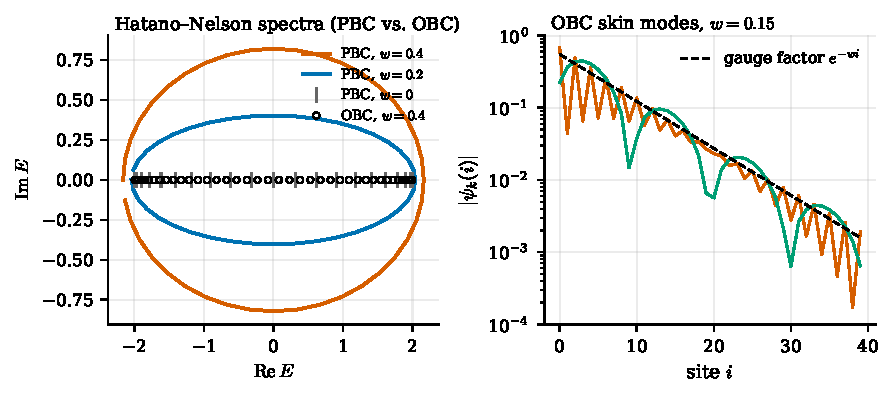
\includegraphics[width=\linewidth]{figs/fig_skin.pdf}
\caption{The skin-obstruction theorem (Theorem~\ref{thm:skin}). Left:
Hatano--Nelson spectra. Nonzero imaginary flux (periodic boundaries,
$w\ne0$) winds the spectrum into a complex loop---no closed process, no
fixed beables; the flux-free cases ($w=0$, or any $w$ with open
boundaries) have real spectra. Right: open-boundary skin modes
$|\psi_k(i)|$ ride the pure-gauge envelope $\ee^{-wi}$ (dashed): the skin
pileup is precisely the beable-preserving metric
$d_i=\ee^{2wi}$ in disguise, exact at finite $N$ and exponentially
degenerate as $N\to\infty$.}
\label{fig:skin}
\end{figure}

%=====================================================================
\section{The broken phase as an open subsystem}
\label{sec:broken}

\subsection{Broken \texorpdfstring{$\PT$}{PT} dynamics is survival-conditioned dynamics}

Write \eqref{eq:dimer} as the balanced gain/loss form
$H=\cos\theta\,\mathbf 1+\ii\sin\theta\,\sigma_z+s\,\sigma_x$. Subtracting
the uniform gain,
\begin{equation}
H_{\rm loss}=H-\ii\sin\theta\,\mathbf 1,
\qquad
\ee^{-\ii Ht}=\ee^{\sin\theta\,t}\,C(t),\quad C(t)=\ee^{-\ii H_{\rm loss}t},
\label{eq:lossframe}
\end{equation}
where $C(t)$ is a contraction (singular values $\le 1$; verified to
machine precision). The notorious broken-phase runaway is thus a scalar
normalization: broken-$\PT$ evolution \emph{is} the no-leak-conditioned
dynamics of a lossy system.

For each $t$ the Halmos dilation \cite{Halmos1950,SzNagy2010}
\begin{equation}
U_{\rm big}(t)=
\begin{pmatrix}
C(t) & \sqrt{\mathbf 1-C(t)C(t)^{\dagger}}\\[2pt]
\sqrt{\mathbf 1-C(t)^{\dagger}C(t)} & -C(t)^{\dagger}
\end{pmatrix}
\label{eq:halmos}
\end{equation}
is exactly unitary with $\Gam_{\rm big}(0)=\mathbf 1_4$. Because the
correspondence requires only per-time unistochasticity---the family need
not compose---$\Gam_{\rm big}(t)=|U_{\rm big}(t)|^{2}$ is an
\emph{ordinary} Barandes indivisible process on four configurations
$\{1,2,a_1,a_2\}$ (two system sites, two ``leaked'' ancilla
configurations), and the reduction
\begin{equation}
\Gam_{\rm red}(t)=|C(t)|^{2}
\label{eq:gred}
\end{equation}
is a sub-stochastic process (column deficits $=$ leak probabilities), valid
at all times in the phase where the closed construction failed totally.
(A unitary-embedding perspective on $\PT$ dynamics---a ``hidden entangled
partner'' restoring lost information---was developed by Kawabata, Ashida,
and Ueda \cite{KAU2017}; the per-time Halmos dilation used here is its
process-level counterpart.)

\subsection{Exact generator: terminal indivisibility}

\begin{theorem}[terminal indivisibility in the broken phase]
\label{thm:terminal}
Let $\tilde\kappa=\sqrt{\sin^{2}\theta-s^{2}}>0$ and set (notation local
to this theorem and its proof)
$c=\cosh\tilde\kappa t$, $\sigma=\sinh(\tilde\kappa t)/\tilde\kappa$,
\[
p=c+\sin\theta\,\sigma,\qquad
q=c-\sin\theta\,\sigma,\qquad
r=s\,\sigma .
\]
Then
\begin{equation}
\Gam_{\rm red}(t)=\ee^{-2\sin\theta\,t}
\begin{pmatrix} p^{2} & r^{2}\\ r^{2} & q^{2}\end{pmatrix},
\qquad
\det\Gam_{\rm red}=\ee^{-4\sin\theta\,t}\,(1-2r^{2}),
\label{eq:gredclosed}
\end{equation}
and the generator $L=\dot\Gam_{\rm red}\Gam_{\rm red}^{-1}$ has the exact
off-diagonal entries
\begin{equation}
L_{12}=\frac{2spr}{1-2r^{2}},
\qquad
L_{21}=\frac{2sqr}{1-2r^{2}} .
\label{eq:generator}
\end{equation}
Consequently:
\begin{itemize}
\item[(i)] the process is P-divisible precisely on $[0,t_c)$ with
$t_c=\tilde\kappa^{-1}\,\mathrm{arcsinh}\!\bigl(\tilde\kappa/(s\sqrt2)\bigr)$,
which is exactly the time at which $\det\Gam_{\rm red}$ crosses zero;
\item[(ii)] $L_{12}<0$ strictly for \emph{all} $t>t_c$: permanent
(terminal) indivisibility;
\item[(iii)] $L_{12}\to-(\sin\theta+\tilde\kappa)$ as $t\to\infty$;
\item[(iv)] $L_{21}$ returns positive at
$t_0=\tilde\kappa^{-1}\,\mathrm{artanh}(\tilde\kappa/\sin\theta)>t_c$:
late-time indivisibility is carried entirely by transitions into the gain
site;
\item[(v)] the same formulas continue to the unbroken phase
($\tilde\kappa\to \ii\kappa$), where
$1-2r^{2}=1-2(s/\kappa)^{2}\sin^{2}\kappa t$ with $(s/\kappa)^{2}>1$
oscillates through zero forever (recurrent indivisibility windows of
period $\pi/\kappa$), and to the exceptional point, where everything is
polynomial with $r=st$ and $t_c=1/(s\sqrt2)$, continuously in $s$.
\end{itemize}
\end{theorem}

\begin{proof}
Since $A=\ii\sin\theta\,\sigma_z+s\sigma_x$ obeys
$A^{2}=(s^{2}-\sin^{2}\theta)\mathbf 1=-\tilde\kappa^{2}\mathbf 1$,
$\ee^{-\ii At}=c\,\mathbf 1-\ii\sigma A$, giving
\eqref{eq:gredclosed} entrywise. With $r'=sc$ and
$p'=\tilde\kappa^{2}\sigma+\sin\theta\,c$ one finds the Wronskian-type
identities
\[
r'p-p'r \;=\; r'q-q'r \;=\; s\,(c^{2}-\tilde\kappa^{2}\sigma^{2}) \;=\; s ,
\]
constants in $t$; inserting them into
$L=\dot{\tilde\Gam}\tilde\Gam^{-1}-2\sin\theta\,\mathbf 1$ (the scalar
factor shifts only the diagonal) yields \eqref{eq:generator}. Statements
(i)--(v) follow by inspection of signs: $p,r>0$ always, $1-2r^{2}$ crosses
zero once (hyperbolic) at $t_c$, $q$ crosses zero once at $t_0>t_c$, and
$L_{12}\to -(\sin\theta+\tilde\kappa)$ from the asymptotics
$c\sim\tilde\kappa\sigma\sim\tfrac12\ee^{\tilde\kappa t}$.
\end{proof}

The predictions are exact against brute-force numerics
(Fig.~\ref{fig:generator}; closed forms to $10^{-14}$, generator to
$10^{-11}$; the observed floor $-1.207$ at $s=0.5$ is
$-(\sin\tfrac\pi4+0.5)=-1.2071$; the observed first indivisible time
$1.35$ on a $0.05$ grid is $t_c=1.3170$).

\begin{figure}[t]
\centering
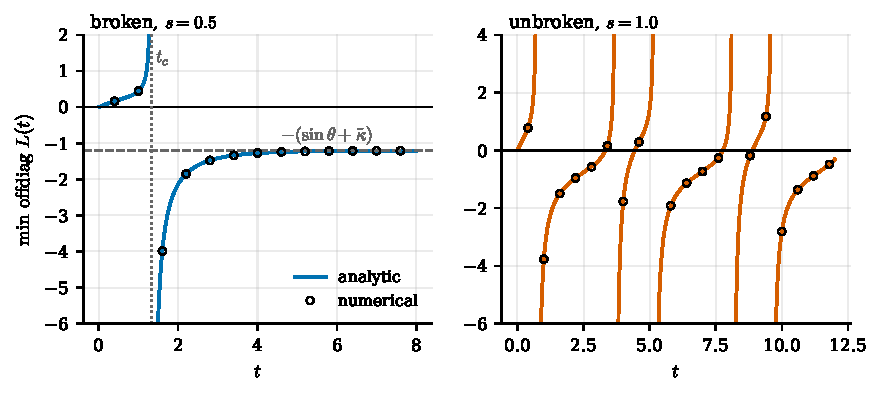
\includegraphics[width=\linewidth]{figs/fig_generator.pdf}
\caption{Minimum off-diagonal entry of the generator
$L(t)=\dot\Gam_{\rm red}\Gam_{\rm red}^{-1}$ of the reduced process
\eqref{eq:gred}: analytic closed forms \eqref{eq:generator} (curves) versus
brute-force numerics (circles). Left: broken phase ($s=0.5$)---divisibility
is lost at $t_c$, exactly where $\det\Gam_{\rm red}$ crosses zero, and
never recovers; the generator approaches the strictly negative floor
$-(\sin\theta+\tilde\kappa)$ (Theorem~\ref{thm:terminal}):
\emph{terminal} indivisibility. Right: unbroken phase ($s=1.0$)---the
same closed forms continued to trigonometric functions give
\emph{recurrent} windows of divisibility and indivisibility at the Rabi
period (curves interrupted where $\det\Gam_{\rm red}$ passes through
zero).}
\label{fig:generator}
\end{figure}

\subsection{The two non-Markovianities dissociate}

For open systems, non-Markovianity is commonly diagnosed by information
backflow (increase of trace/total-variation distance between two
evolutions) \cite{BLP2009,RHP2010,BreuerReview2016}. On the classical
marginal with the leak recorded as a third outcome, the total-variation
distance is monotone in \emph{both} phases (no classical backflow at all);
on the survival-conditioned (post-selected) process, the late-window
backflow vanishes identically for every broken $s$ and jumps at the EP
(e.g.\ $0.000\to1.32$ across $s_*=0.7071$ at $s=0.72$, window
$t\in[20,40]$)---the stochastic-level analogue of the
reversible--irreversible criticality of information flow established for
$\PT$ systems by Kawabata, Ashida, and Ueda \cite{KAU2017}. Meanwhile,
Barandes indivisibility is present in \emph{both}
phases; what changes at the EP is its temporal structure, recurrent
$\leftrightarrow$ terminal (the terminal-indivisibility theorem,
Theorem~\ref{thm:terminal}). Figure
\ref{fig:dissociation} contrasts the two diagnostics across the
transition: the backflow order parameter switches at the EP, while the
indivisibility onset $t_c(s)$ is finite and \emph{continuous} through it.

\begin{figure}[t]
\centering
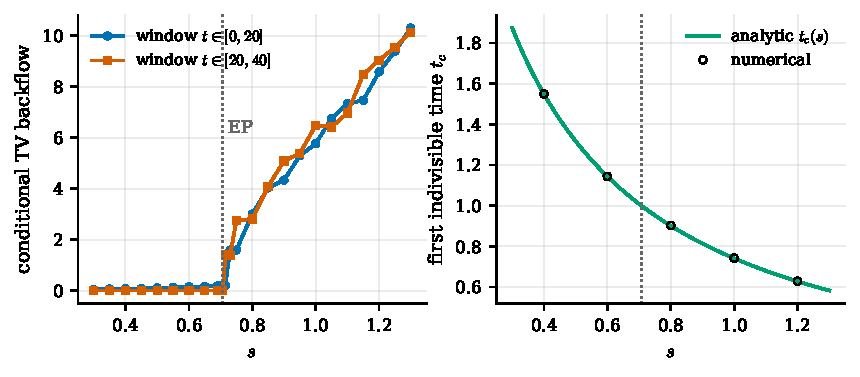
\includegraphics[width=\linewidth]{figs/fig_dissociation.pdf}
\caption{The two non-Markovianities across the $\PT$ transition
(EP at $s_*=\sin\tfrac\pi4\approx0.707$, dotted line). Left: conditional
total-variation backflow in an early ($t\in[0,20]$) and a late
($t\in[20,40]$) window; the late-window backflow vanishes identically in
the broken phase and switches on at the EP (the apparent smoothness just
above $s_*$ is the diverging Rabi period $\pi/\kappa$ meeting the finite
window). Right: the first indivisible time $t_c(s)$ of
Theorem~\ref{thm:terminal}, analytic in both phases and continuous
through the EP (circles: numerical onset). Indivisibility is present on
both sides; backflow is not.}
\label{fig:dissociation}
\end{figure}

Thus the broken phase is \emph{backflow-Markovian in the late window
yet permanently Barandes-indivisible}:
the two notions genuinely dissociate, indivisibility being strictly finer.
That the relation between divisibility- and information-flow-based
notions of Markovianity is subtle for quantum channels---equivalent
for invertible maps \cite{ChruscinskiRS2018}, genuinely inequivalent
for noninvertible ones \cite{Rivas2022}---is known; the $\PT$ dimer
makes the dissociation exact,
phase-locked, and---in the broken phase---permanent, at the level of the
classical configuration process.
A closed Hermitian system, being quasi-periodic, can only be recurrently
indivisible; terminal indivisibility with monotone leak is the stochastic
signature of the broken phase. (At $n=2$ every lossy two-site Hamiltonian
\emph{with degenerate site frequencies} is a shifted $\PT$ dimer, so
there ``overdamped open dynamics'' and ``broken
$\PT$'' coincide; a detuned pair adds a real $\sigma_z$ component the
$\PT$ form does not carry.)

%=====================================================================
\section{The exceptional point is a coordinate singularity}
\label{sec:ep}

At $s_*=\sin\theta$ the dimer is defective (a Jordan block; numerically
$\mathrm{rank}(H-\cos\theta\,\mathbf 1)=1$), the naive process grows
polynomially ($|U|^2$ column sums $\sim t^{2}$; fitted exponent $1.95$),
and the two-dimensional space of Hermitian intertwiners consists of one
\emph{singular positive-semidefinite rank-one ray} and one indefinite
direction: the positive-definite cone is exited exactly through its
boundary, and $\rho$ does not exist.

Approaching from the unbroken side, $s=s_*(1+\varepsilon)$,
$\kappa\simeq\sin\theta\sqrt{2\varepsilon}$, we find clean power laws
(Fig.~\ref{fig:ep}; log--log fits over $\varepsilon=10^{-1}\dots10^{-7}$,
all within $\pm0.0025$):
\begin{center}
\begin{tabular}{lll}
\toprule
quantity & scaling & fitted slope\\
\midrule
$\mathrm{cond}(\eta)$ & $\varepsilon^{-1}\sim\kappa^{-2}$ (Petermann
\cite{Petermann1979}) & $-0.998$\\
$\mathrm{cond}(\rho)$ (beable-map anisotropy) & $\varepsilon^{-1/2}\sim\kappa^{-1}$ & $-0.499$\\
$\norm{\Gam_{\varepsilon}(t)-\mathbf 1}$ at fixed $t$ & $\varepsilon\sim(\kappa t)^{2}$ & $+0.999$\\
\bottomrule
\end{tabular}
\end{center}
\begin{figure}[t]
\centering
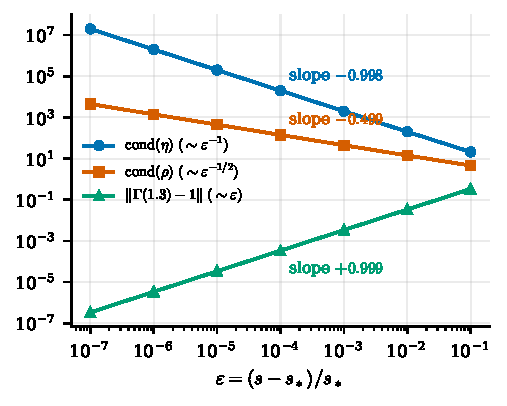
\includegraphics[width=0.55\linewidth]{figs/fig_ep_scaling.pdf}
\caption{Collapse of the closed-system (metric) description approaching
the exceptional point from the unbroken side, $s=s_*(1+\varepsilon)$. The
metric condition number diverges with the Petermann scaling
$\varepsilon^{-1}\sim\kappa^{-2}$, the beable-map anisotropy as
$\varepsilon^{-1/2}\sim\kappa^{-1}$, while the metric-corrected process at
fixed laboratory time \emph{freezes},
$\norm{\Gam_\varepsilon(t)-\mathbf 1}\sim\varepsilon\sim(\kappa t)^2$.}
\label{fig:ep}
\end{figure}

At fixed laboratory time the metric-corrected process therefore
\emph{freezes}: $h\to\cos\theta\,\mathbf 1$ and
$\Gam_\varepsilon(t)\to\mathbf 1$. A regularized lab-time limit exists but
is trivial---and is not the EP dynamics, which grows like $t^{2}$. On the
critically rescaled clock $\tau=\kappa t$ the process converges (to
$10^{-10}$ between $\varepsilon=10^{-4}$ and $10^{-6}$) to the universal
indivisible Rabi process
\begin{equation}
\Gam_{\lim}(\tau)=
\begin{pmatrix}\cos^{2}\tau & \sin^{2}\tau\\ \sin^{2}\tau & \cos^{2}\tau
\end{pmatrix},
\end{equation}
with Rabi axis exactly $\sigma_x$; but the beable map identifying its
states with the original configurations diverges
($\mathrm{cond}\,\rho\sim\kappa^{-1}$): the survivor is abstract.

By contrast, every open-system quantity of Sec.~\ref{sec:broken}
(reduced-process entries, survival, indivisibility generator floor) varies
smoothly and monotonically through $s_*$. \emph{The EP is a singularity of
the similarity-to-Hermitian dictionary, not of the stochastic process}:
existence of an indivisible process is governed by the dilation, and the
deflation of Proposition~\ref{prop:deflation} fails at the EP only because
its coordinates do.

%=====================================================================
\section{The Pais--Uhlenbeck oscillator}
\label{sec:pu}

The PU Lagrangian
$L=\tfrac{\gamma}{2}\bigl[\ddot x^{2}-(\omega_1^{2}+\omega_2^{2})\dot
x^{2}+\omega_1^{2}\omega_2^{2}x^{2}\bigr]$
has the Ostrogradski Hamiltonian (with $q_1=x$, $q_2=\dot x$)
\begin{equation}
H_{\rm PU}=p_1q_2+\frac{p_2^{2}}{2\gamma}
+\frac{\gamma}{2}(\omega_1^{2}+\omega_2^{2})q_2^{2}
-\frac{\gamma}{2}\omega_1^{2}\omega_2^{2}q_1^{2},
\label{eq:ostro}
\end{equation}
which is \emph{Hermitian} on the real configuration space $(x,\dot x)$,
with the ghost spectrum
$E=\omega_1(n_1+\tfrac12)-\omega_2(n_2+\tfrac12)$: real, unbounded below
\cite{PaisUhlenbeck1950,BenderMannheim2008}.

\subsection{The ghost realization is a valid fixed-beable process}

On a discretized $(x,\dot x)$ grid ($44^{2}=1936$ configurations, spectral
derivatives, $\omega_1=1$, $\omega_2=0.5$, $\gamma=1$) the operator
\eqref{eq:ostro} is exactly Hermitian; $\Gam=|U|^{2}$ is doubly stochastic
to $2\times10^{-14}$ and genuinely indivisible
($\norm{\Gam(2t)-\Gam(t)^{2}}\approx2.7$); Hermiticity makes (K1)--(K4)
hold trivially with $\eta=\mathbf 1$, so the beables are fixed. The
realization is validated dynamically: Ehrenfest is exact for quadratic
Hamiltonians, and $\avg{x(t)}$ tracks the exact classical fourth-order
trajectory to $3\times10^{-3}$ over half the evolution window (residual
from packet tails at the box walls; Fig.~\ref{fig:pu}).

\begin{figure}[t]
\centering
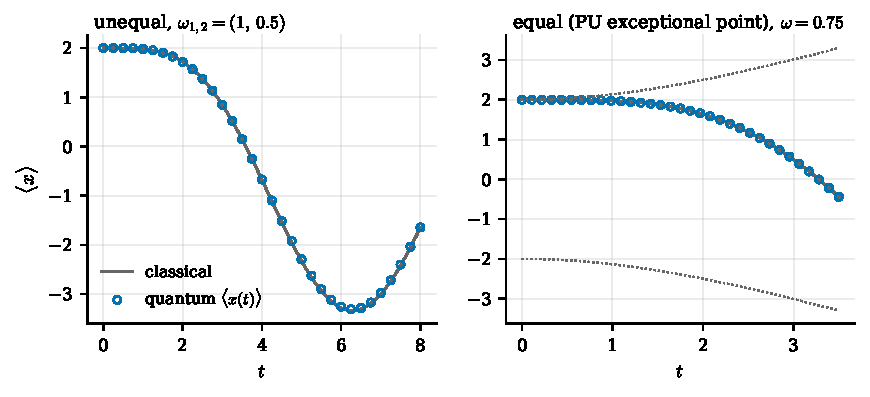
\includegraphics[width=\linewidth]{figs/fig_pu_ehrenfest.pdf}
\caption{The ghost realization of the free Pais--Uhlenbeck oscillator as
a stochastic process on physical configurations: $\avg{x(t)}$ of the grid
process (circles) versus the exact classical fourth-order trajectory
(line). Left: unequal frequencies. Right: equal frequencies---the PU
exceptional point---where the classical normal-mode matrix is defective
and the solution grows secularly, $x(t)=2\cos\omega t+\omega t\sin\omega
t$ (dotted: envelope $\pm\sqrt{4+(\omega t)^2}$); the Hermitian
realization crosses the point smoothly while $\Gam$ remains exactly
doubly stochastic.}
\label{fig:pu}
\end{figure}

The spectrum of the grid operator
runs from $-26$ to $+140$ and is \emph{completely irrelevant to the
process}: at the free level the Ostrogradski ghost is an energy-accounting
pathology, invisible to the stochastic representation.

At equal frequencies (the PU exceptional point) the classical normal-mode
matrix is defective (eigenvector condition number $\sim10^{8}$; secular
$t\sin\omega t$ growth), yet the Hermitian realization passes through
smoothly: $\avg{x(t)}$ tracks $2\cos\omega t+\omega t\sin\omega t$ to
$9\times10^{-4}$ and $\Gam$ stays exactly doubly stochastic---the
PU-scale confirmation of Sec.~\ref{sec:ep}.

\subsection{The no-ghost quantization exits the sample space}

Mannheim's positive spectrum requires re-quantizing the ghost mode with a
vacuum satisfying $b^{\dagger}\Omega=0$, i.e.\ $\Omega\propto\ee^{+y^{2}/2}$:
normalizable only on a rotated contour \cite{BenderMannheim2008}. This is
a \emph{domain change}, not a similarity (a similarity cannot flip the
spectrum), and it has no shadow at any truncation: the null vector of the
truncated $b$ is $\ket{0}$ at every $N$ (the true vacuum,
truncation-stable), while the null vector of the truncated $b^{\dagger}$
is $\ket{N-1}$, pinned to the truncation edge and escaping to infinite
energy; restricted to any fixed low-energy sector,
$\sigma_{\min}(b^{\dagger})=1$ exactly. The contour-rotation operator
$R=\ee^{(\pi/2)D}$, $D=\tfrac12(yp+py)=\tfrac{\ii}{2}(a^{\dagger2}-a^{2})$,
has $\log_{10}\mathrm{cond}(R_N)$ growing at $\approx1.2$ decades per Fock
level ($53$ decades at $N=48$), so the would-be metric
$\sim(RR^{\dagger})^{-1}$ is unbounded with unbounded inverse: the
Sec.~\ref{sec:ep} collapse at every scale at once, with no
critical-rescaling survivor.

\emph{Verdict.} The stochastic--quantum correspondence and the $\PT$
no-ghost construction resolve the free ghost in incompatible currencies:
Barandes keeps real beables and pays in negative energies; Mannheim buys
positive energies and pays with the sample space itself. (A related
construction by Salvio and Strumia \cite{SalvioStrumia2016} obtains
positive energies and normalizable wave functions at the price of a
negative-norm configuration-space inner product---again incompatible with
a probability measure over configurations.) The dynamics-dependent beable
rotation of Sec.~\ref{sec:deflation} escalates, in the PU limit, to beable
\emph{non-existence}.

%=====================================================================
\section{Interacting ghosts: conservative, transient, explosive}
\label{sec:interacting}

Does the ghost instability, once interactions are switched on, become a
\emph{stochastic} pathology? The answer arrives in stages.

\subsection{Quadratic interactions: a valid process turns transient}

Consider the Hermitian cascade Hamiltonian
\begin{equation}
H=\omega_1 a^{\dagger}a-\omega_2 b^{\dagger}b
+g\,(a^{\dagger}b^{\dagger}+ab),
\label{eq:cascade}
\end{equation}
whose normal twin has $+\omega_2 b^{\dagger}b$. The Heisenberg mode matrix
has eigenvalues
$\bar\omega\pm\sqrt{\delta^{2}/4-g^{2}}$ (ghost; $\delta=\omega_1-\omega_2$,
$\bar\omega=(\omega_1+\omega_2)/2$), so the ghost sign collapses the
instability threshold from the \emph{sum} frequency, $g>(\omega_1+\omega_2)/2$
(normal), to the \emph{difference} frequency, $g>|\omega_1-\omega_2|/2$:
zero at resonance. At resonance the vacuum cascades with the exact
two-mode-squeezing laws
\begin{equation}
\avg{n_1(t)}=\avg{n_2(t)}=\sinh^{2}(gt),
\qquad
P\bigl(n_1\le K\bigr)=1-\tanh^{2K+2}(gt)\;\longrightarrow\;0 ,
\label{eq:cascadelaws}
\end{equation}
both matched numerically to $\sim$4 decimals in the resolved regime
($\langle n\rangle\lesssim$ a few, before the $34^2$ Fock truncation
sets in at the last tabulated time) (Fig.~\ref{fig:cascade};
Fock truncation $34^2$, $g=0.15$; detuned growth consistent with
$(g^{2}/\kappa^{2})\sinh^{2}\kappa t$, $\kappa=\sqrt{g^{2}-\delta^{2}/4}$),
while $\Gam$ remains doubly stochastic to $2\times10^{-14}$ and the energy
books stay exactly balanced ($E_{\rm normal}=+8.301$,
$E_{\rm ghost}=-8.301$, $\avg{H}=0$ conserved).

\begin{figure}[t]
\centering
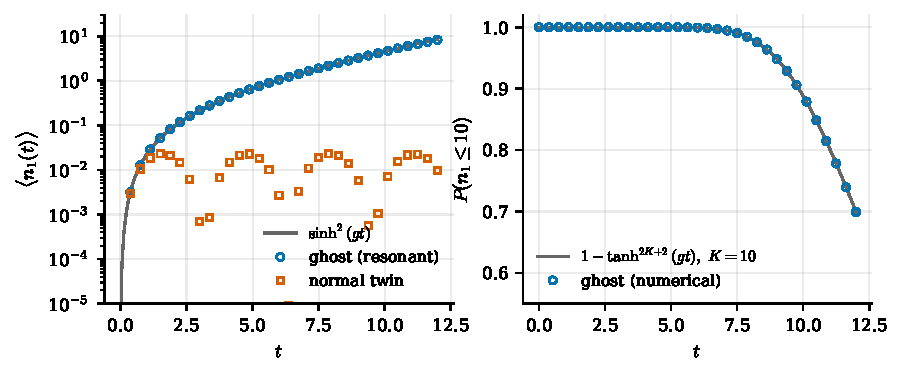
\includegraphics[width=\linewidth]{figs/fig_cascade.pdf}
\caption{The quadratic ghost cascade \eqref{eq:cascade} at resonance
($\omega_1=\omega_2$, $g=0.15$): a valid, exactly doubly stochastic
process that is \emph{transient}. Left: occupation growth
$\avg{n_1(t)}=\sinh^2(gt)$ (line: exact law; circles: Fock-space
numerics), while the normal-sign twin (squares) stays bounded below
$3\times10^{-2}$---the instability threshold collapses from the sum
to the difference frequency. Right: escape from the occupation ball $n_1\le10$
follows the exact two-mode-squeezing law
\eqref{eq:cascadelaws}.}
\label{fig:cascade}
\end{figure}

\emph{Vacuum decay is a
configuration-space cascade with balanced energy books}: the process is
valid and indivisible but \emph{transient}---it permanently escapes every
finite region at rate $2g$---which is the first stage at which the ghost
becomes visible in the process's own currency.

\subsection{Malicious nonlinearities: finite-time escape}

Classically, the ghost pair
$\tfrac12(p_1^{2}+\omega_1^{2}x_1^{2})-\tfrac12(p_2^{2}+\omega_2^{2}x_2^{2})
+\lambda x_1^{2}x_2^{2}$ is mostly bounded at moderate amplitude (benign
islands \cite{Smilga2005}), while the quartic PU,
\begin{equation}
\ddddot{x}+(\omega_1^{2}+\omega_2^{2})\ddot
x+\omega_1^{2}\omega_2^{2}x=\frac{4\lambda}{\gamma}x^{3},
\end{equation}
exhibits robust \emph{finite-time} blowup for both signs of $\lambda$ at
every amplitude tested ($t_*=3.3$--$6.9$); for $\lambda>0$ the dominant
balance is $x\sim A(t_*-t)^{-2}$, $A=\sqrt{30\gamma/\lambda}$ (the
$\lambda<0$ escape proceeds by a different mechanism, taken up in
Sec.~\ref{sec:multiD}). Quantum-mechanically,
a lattice can transport the accelerating wavefront only while the required
classical speed stays below the Nyquist momentum $\pi/\Delta x$; box-size
drifts of the leak onset correlate exactly with
$v_{\rm cl}(\text{edge})/k_{\max}=1.4,2.4,3.4$ and are lattice
confinement, not physics (a fact that itself echoes
Sec.~\ref{sec:dictionary}: a non-\esa{} operator has no faithful finite
truncation). In the resolved regime, quantum probability arrives at every
probed radius at times bounded by the classical finite-time law, with bulk
weight, while the free control never passes $r\approx7$.

In the standard vocabulary of stochastic processes, the hierarchy is:
free/normal-sign $=$ \emph{conservative}; ghost with quadratic (or benign
nonlinear) interaction $=$ \emph{transient}; ghost with malicious
nonlinearity $=$ \emph{explosive} (mass leaves the state space in finite
time). The Ostrogradski ghost is a recurrence-classification problem.
Complementary operator-theoretic and dynamical stability results for
interacting
ghosts---the global-stability classification program of Errasti
D\'iez, Gaset Rif\`a, and Staudt \cite{ErrastiDiez2024} and its
multidimensional classical-scattering extension by
Held \cite{Held2025}, conserved quantities with discrete
spectrum \cite{Deffayet2026},
and exact moment bounds \cite{EwasiukProfumo2026}---identify
interaction
structures in which the cascade is arrested; in the present language,
those are mechanisms enforcing recurrence (none of these works uses
the stochastic/recurrence currency itself).

%=====================================================================
\section{The explosion dictionary}
\label{sec:dictionary}

The mechanism of malicious escape is one-dimensional: motion along a
direction where the effective potential falls super-quadratically. For
this mechanism the correspondence between the three descriptions can be
made a theorem.

\begin{theorem}[explosion dictionary, 1D mechanism model]
\label{thm:dictionary}
Let $H=\tfrac12 p^{2}+V$ on the line with an escaping end
($V\to-\infty$ eventually monotonically and $C^{1}$ with
$|V'|\,|V|^{-3/2}$ bounded, the standard regularity under which the
limit-point/limit-circle criteria below apply---the mechanism model;
Rauch--Reed's oscillatory one-dimensional counterexamples
\cite{RauchReed1973} show this hypothesis cannot be dropped), and
define the classical time of flight
$T(E)=\int^{\infty}\dd x/\sqrt{2(E-V(x))}$.
\begin{itemize}
\item[(1)] If $T=\infty$ (e.g.\ $V\gtrsim-Kx^{2}$), the end is limit
point, and---with the non-escaping end confining, hence also limit
point---$H$ is \esa{} \cite{ReedSimon2}, there is a unique unitary $U(t)$
and a unique conservative process.
\item[(2)] If $T<\infty$ (e.g.\ $V\lesssim -Kx^{2+\epsilon}$), the end is
limit circle \cite{ReedSimon2}, by the (WKB-asymptotic) identity
\begin{equation}
|\psi_{\pm}(x)|^{2}\;\approx\;\bigl[2(E-V(x))\bigr]^{-1/2}
\quad\Longrightarrow\quad
\int^{\infty}\!|\psi_{\pm}|^{2}\,\dd x \;\approx\; T :
\label{eq:onelineidentity}
\end{equation}
\emph{the deficiency solution's norm is, to WKB accuracy, the
classical time of flight} (the limit-point/limit-circle dichotomy
itself is exact; the identity quantifies it semiclassically).
Consequently:
\begin{itemize}
\item[(a)] there is no canonical unitary dynamics: self-adjoint extensions
form a $U(1)$ family per escaping end ($U(2)$ for two ends, including
completions that transmit through infinity), i.e.\ boundary data at
infinity \cite{ReedSimon2};
\item[(b)] every extension is conservative but returns probability from
infinity after the finite classical round trip; its spectrum is discrete
with local spacing, semiclassically,
$\Delta E\simeq\pi/T_{\rm cross}(E)$, $T_{\rm cross}$ the
classical traversal time;
\item[(c)] the regulator-independent object is the minimal (Feller)
semigroup \cite{Feller1952}: a sub-stochastic, \emph{explosive} process
losing mass at the classical escape rate;
\item[(d)] one integral decides classical completeness, quantum essential
self-adjointness (Weyl \cite{Weyl1910}), and stochastic conservativity
(Feller exit boundary).
\end{itemize}
\end{itemize}
\end{theorem}

The rigorous inputs are Weyl's alternative and the limit-point/limit-circle
criteria of \cite{ReedSimon2} (Thms.~X.8--X.10); the WKB norms and the
semiclassical spacing law are used at their standard validity.

Numerical verification (representative $V=-x^{4}$, marginal control
$V=-x^{2}$): the spacing law matches to $3.5\%$ or better in all eight
$(V,L)$ cases tested and to $0.3\%$ at the largest box for
$V=-x^{4}$ (Table~\ref{tab:spacing}); the eigenvalue nearest $E=10$
(a tracked-level probe, distinct from the spacing window at $E=11$)
sweeps
erratically with the wall position (no completion has an $L\to\infty$
limit) while the spacing is stable; a 1D absorbing-boundary evolution
(where the lattice barrier is beatable) absorbs $98.6$--$98.8\%$ of the
probability by $t=1$ \emph{independently of box size}, with onset
saturating toward the classical arrival ($T_{\rm esc}=0.4635$;
Fig.~\ref{fig:explosion}, left); and two completions of the same
$H$---Dirichlet wall versus periodic identification---both revive
$\approx95\%$ of the probability after the finite round trip but from
\emph{opposite sides} (reflection versus a $+\infty\to-\infty$
``wormhole''; Fig.~\ref{fig:explosion}, right), an observable difference
encoded nowhere in $H$.

\begin{figure}[t]
\centering
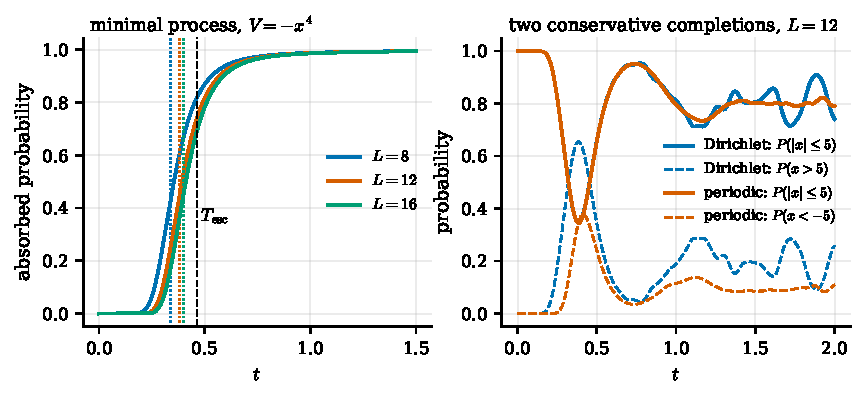
\includegraphics[width=\linewidth]{figs/fig_explosion.pdf}
\caption{Explosion and its completions for $V=-x^4$
(the explosion dictionary, Theorem~\ref{thm:dictionary}). Left: the
minimal (absorbed) process is
box-independent---the absorbed probability for $L=8,12,16$ collapses onto
one curve with onset tracking the classical arrival at each absorber edge
(dotted verticals) and saturating at the finite escape time
$T_{\rm esc}$ (dashed): probability reaches infinity at finite time.
Right: two conservative completions of the same symmetric operator. Both
revive $\approx95\%$ of the probability after the finite round trip
``through infinity,'' but the Dirichlet wall returns it from the right
(reflection) while the periodic identification returns it from the left
(transmission, $+\infty\to-\infty$): the completion is boundary data at
infinity, not physics contained in $H$.}
\label{fig:explosion}
\end{figure}

\begin{table}[t]
\centering
\begin{tabular}{lcccc}
\toprule
 & \multicolumn{2}{c}{$V=-x^{4}$ (malicious)} &
 \multicolumn{2}{c}{$V=-x^{2}$ (marginal)}\\
$L$ & measured $\Delta E$ & $\pi/T_{\rm cross}$ &
measured $\Delta E$ & $\pi/T_{\rm cross}$\\
\midrule
$6$  & $2.559$ & $2.609$ & $1.619$ & $1.640$\\
$9$  & $2.365$ & $2.449$ & $1.290$ & $1.289$\\
$12$ & $2.345$ & $2.377$ & $1.106$ & $1.112$\\
$16$ & $2.318$ & $2.325$ & $0.964$ & $0.975$\\
\bottomrule
\end{tabular}
\caption{Level spacing of the wall-regularized completions near $E=11$
versus the classical law $\pi/T_{\rm cross}(E,L)$. For the malicious
potential the traversal time to infinity is finite, so the spacing
saturates: every conservative completion reflects off infinity at a finite
recurrence time. For the marginal control the spacing decays toward the
continuum.}
\label{tab:spacing}
\end{table}

%=====================================================================
\section{Multidimensional theory: channels and the \texorpdfstring{$S$}{S}-matrix at infinity}
\label{sec:multiD}

The naive dictionary ``classical incompleteness
$\Leftrightarrow$ quantum non-self-adjointness'' fails in general
beyond the monotone one-dimensional mechanism model: Rauch and Reed
constructed one-dimensional counterexamples in both directions
\cite{RauchReed1973}, and in $n\ge2$ the correct structure is
channel-wise. Throughout,
$H$ is defined on $C_0^{\infty}$ and deficiency indices refer to its
closure.

\begin{theorem}[quadratic ghosts are safe]
\label{thm:quadratic}
Every at-most-quadratic Hamiltonian on $\mathbb R^{n}$---including the
indefinite cascade \eqref{eq:cascade} at any coupling, even in the
unstable phase, and the free PU operator \eqref{eq:ostro}---is \esa{} on
the span of Hermite functions.
\end{theorem}

\begin{proof}
A quadratic $H$ maps Hermite level $N$ into levels $\le N+2$ with
coefficients $O(N)$, so
$\norm{H^{n}\psi_N}\le(2C)^{n}\,(N/2+n)!/(N/2)!$
and $\sum_n t^{n}\norm{H^{n}\psi_N}/n!$ converges for small $t$: every
Hermite function is an analytic vector. Nelson's analytic vector theorem
\cite{Nelson1959} applies.
\end{proof}

Thus instability never breaks uniqueness or conservativity: the
transient/explosive dichotomy of Sec.~\ref{sec:interacting} is rigorous on
the transient side.

\begin{theorem}[channel additivity of deficiency]
\label{thm:channels}
Let $H=h_1\otimes\mathbf 1+\mathbf 1\otimes h_{\perp}$ on
$L^{2}(\mathbb R\times\mathbb R^{m})$, with $h_1=\tfrac12p^{2}+V_1$
super-quadratically falling at every end (limit circle at both
$\pm\infty$) and $h_{\perp}$ self-adjoint
with orthonormal eigenbasis $\{\varphi_n,E_n\}$. Then for every $n$ and
every solution $u$ of $\bigl(h_1-(\pm\ii-E_n)\bigr)u=0$ (all of which are
$L^{2}$, since the limit-circle property at each end is independent of
the spectral
parameter), $u\otimes\varphi_n\in\ker(H^{*}\mp\ii)$. Hence the deficiency
indices of $H$ are $(\infty,\infty)$.
\end{theorem}

\begin{proof}
$H^{*}$ acts distributionally, and
$H(u\otimes\varphi_n)
=\bigl((\pm\ii-E_n)u\bigr)\otimes\varphi_n+E_n\,u\otimes\varphi_n
=\pm\ii\,u\otimes\varphi_n\in L^{2}$,
so $u\otimes\varphi_n\in D(H^{*})$ and is a deficiency vector; vectors
with different $n$ are orthogonal.
\end{proof}

\begin{corollary}
\label{cor:central}
$-\tfrac12\Delta-c|x|^{\alpha}$ on $\mathbb R^{d}$ with $\alpha>2$ has
deficiency indices $(\infty,\infty)$ (partial-wave separation; the
centrifugal terms are subquadratic).
\end{corollary}

\begin{theorem}[non-separable channel mixing]
\label{thm:kato}
Let $H_0=\tfrac12p_2^{2}-|x_2|^{\alpha}+h_{\perp}(x_1)$, $\alpha>2$, and
$B=\mu f(x_1)g(x_2)$ with $f,g$ bounded and real-valued. Then
$H_0+B$ has the same
(infinite) deficiency indices as $H_0$, while $B$ genuinely mixes the
transverse channels.
\end{theorem}

\begin{proof}
Bounded symmetric perturbations preserve deficiency indices
\cite{KatoBook}.
\end{proof}

\emph{Physical content.} The conservative completions of a malicious
multidimensional ghost are parametrized by unitaries between
infinite-dimensional deficiency spaces: a genuine \emph{$S$-matrix at
infinity}, which may scramble the transverse state upon ``reflection from
infinity''. Numerically (four-channel model, $V_1=-|x|^{5/2}$, bounded
mixing): the wall-regularized level count in a window matches the channel
sum $\sum_n\int T_{\rm cross}(E-E_n,L)\,\dd E/\pi$ (34 vs 32.3 at $L=8$;
37 vs 37.1 at $L=12$), at $\mu=0$ the spectrum is exactly a union of
shifted 1D ladders (deviation $10^{-12}$), switching on the bounded
coupling leaves the counts essentially unchanged ($34\to34$ at $L=8$,
$37\to36$ at $L=12$, a one-level window-edge shift within count
granularity; Kato stability made visible)---and a
packet sent to infinity in the transverse ground state returns as a
channel mixture \emph{whose content depends on where infinity was
regularized} (Fig.~\ref{fig:channels}): fractions
$(0.583,0.346,0.058,0.014)$ for $L=6$ versus $(0.401,0.421,0.143,0.035)$
for $L=9$, with $96\%/93\%$ of the probability returning at the classical
round-trip times.

\begin{figure}[t]
\centering
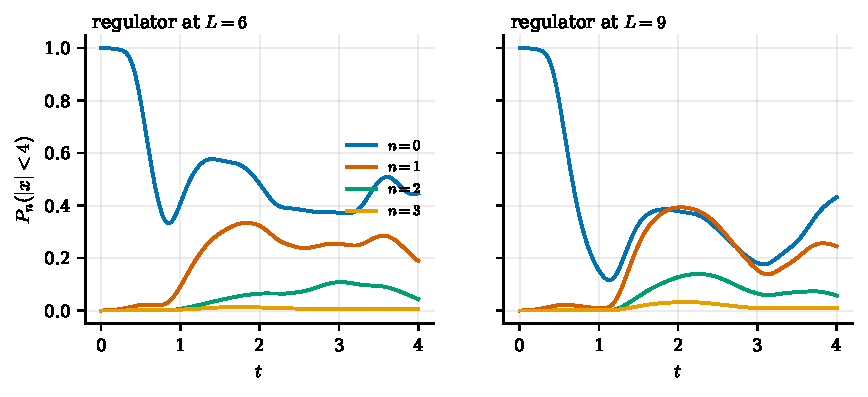
\includegraphics[width=\linewidth]{figs/fig_channels.pdf}
\caption{The $S$-matrix at infinity made visible (four-channel malicious
model of the bounded-mixing theorem, Theorem~\ref{thm:kato}).
Channel-resolved probability in the
interior region $|x|<4$ for a packet launched toward infinity in the
transverse ground state $n=0$. The packet reflects off the regulator and
returns as a channel \emph{mixture}; comparing the two regulator
positions ($L=6$, left; $L=9$, right), the returned mixture differs
substantially. In the $L\to\infty$ limit the reflection law is a genuine
unitary between infinite-dimensional deficiency spaces
(the channel-additivity theorem, Theorem~\ref{thm:channels}):
conservative completions scramble the
transverse state with data injected at infinity.}
\label{fig:channels}
\end{figure}

\begin{remark}[an obstruction specific to ghosts]
For indefinite $H_0=h_1\otimes\mathbf 1+\mathbf 1\otimes h_\perp$ with
$h_1$ unbounded below, transverse observables are \emph{not}
$H_0$-bounded: joint spectral points $(\lambda,\mu)$ with
$\lambda\approx-\mu$ make $\norm{H_0\psi}$ small while
$\norm{h_\perp\psi}$ is large. The standard Kato--Rellich transfer
therefore fails even for mildly unbounded couplings---a second,
ghost-specific obstruction beyond non-separability.
\end{remark}

\begin{openproblem}
\label{op:pu}
Determine the deficiency indices of the exact quartic Pais--Uhlenbeck
operator, $H_{\rm PU}+\lambda q_1^{4}$ of \eqref{eq:ostro}, and of the
ghost pair with coupling $\lambda x_1^{2}x_2^{2}$, on
$C_0^{\infty}(\mathbb R^{2})$. Both escape the hypotheses above (unbounded
diagonal coupling; degenerate/indefinite kinetic form). Either outcome is
significant: infinite deficiency would complete the explosion dictionary
for the physical operators, while essential self-adjointness would be a
``quantum completion'' in the sense of \cite{RauchReed1973}---interactions
curing the ghost's explosion.
\end{openproblem}

\emph{Numerical evidence.} A regulator-dependence campaign (Fock-space
compressions, which regulate position and momentum symmetrically---the PU
escape accelerates without bound---with the matched-eigenvalue-drift
diagnostic calibrated on limit-circle, continuous-spectrum, and discrete
essentially-self-adjoint controls, and on the free PU operator as the
two-dimensional baseline) points to a split verdict. The quartic PU shows
persistent $O(1)$ drift that does not decay with truncation, at two
different basis scales---the limit-circle signature, at $\sim$5$\times$
the free-PU baseline: evidence \emph{against} essential self-adjointness,
i.e.\ for the explosion dictionary applying to the physical operator. The
ghost pair with $\lambda>0$ sits at the essentially-self-adjoint baseline,
as predicted by its Born--Oppenheimer channels
$W_n(x_2)=\tfrac12\omega_2^{2}x_2^{2}-(n+\tfrac12)
\sqrt{\omega_1^{2}+2\lambda x_2^{2}}$, all of which are confining.
Unexpectedly, so does the classically malicious $\lambda<0$ ghost
pair---tentative evidence of a genuine Rauch--Reed-type quantum
completion, in which zero-point energy walls off the narrow classical
escape valley. Evidence, not proof; but it sharpens the problem: prove
deficiency for the quartic PU by quasi-mode construction along its escape
channel, and test the quantum-completion hypothesis for the ghost pair
with valley-adapted bases. (Deficiency indices of related
polynomial-oscillator operators---higher-order squeezing---have recently
been computed rigorously, including cases where added terms
\emph{restore} essential self-adjointness \cite{FischerBL2026}: an
operator-theoretic precedent for completion by interaction.)

The drift verdict for the quartic PU can, in fact, be given structural
support, together with a falsifiable sign prediction:

\begin{proposition}[displaced-oscillator identity (exact) and
channelization (to $O(k^2)$) of the quartic PU]
\label{prop:bo}
In the Fourier-rotated representation ($p_1\to y$, $q_1\to-p_y$), the
displaced-oscillator unitary $U=\exp[-\ii\,y\,p_2/(\gamma\Omega)]$,
$\Omega=\omega_1^2+\omega_2^2$, gives \emph{exactly}
\begin{equation}
U\,(H_{\rm PU}+\lambda q_1^4)\,U^{\dagger}
=T\!\Bigl(p_y+\frac{p_2}{\gamma\Omega}\Bigr)
+\frac{p_2^{2}}{2\gamma}+\frac{\gamma\Omega}{2}q_2^{2}
-\frac{y^{2}}{2\gamma\Omega},
\qquad
T(p)=\lambda p^{4}-\frac{\gamma\Omega_0^{2}}{2}p^{2},
\end{equation}
with $\Omega_0^2=(\omega_1\omega_2)^2$ (verified in Fock space via the
terminating Baker--Campbell--Hausdorff series to $10^{-9}$). The
mode-2-diagonal (channel) part is, in the $k=p_y$ representation and up
to $O(k^{2})$ corrections, \emph{minus} the Schr\"odinger operator
$\hat p^{2}/(2\gamma\Omega)-\lambda k^{4}+(\gamma\Omega_0^{2}/2)k^{2}$;
interchannel couplings are polynomial of degree $\le3$ in $k$,
subordinate to the quartic diagonal. Hence for $\lambda>0$ every channel
is limit circle (finite channel time of flight: $1.74$ for the parameters
used here), and channel additivity as in Theorem~\ref{thm:channels}
argues for deficiency indices $(\infty,\infty)$---with the stability
question settled at every finite channel number by the finite-channel
stability theorem (Theorem~\ref{thm:stability}) below. For
$\lambda<0$ every channel is (minus) a confining operator: quantum
completion predicted, \emph{despite} classical finite-time blowup at both
signs.
\end{proposition}

The sign prediction is confirmed by the drift diagnostic: the classically
explosive $\lambda<0$ quartic PU sits near the essentially-self-adjoint
baseline (ratios $0.17$--$0.46$ at two basis scales, none leaving
the essentially-self-adjoint baseline band), separated from the
$\lambda>0$ limit-circle signature
(the extended truncations give $O(1)$ ratios---$3.77$ at
$N=48{\to}56$, $1.06$ at $N=56{\to}64$---several times to an order
of magnitude
above the ${\sim}0.2$ e.s.a.\ baseline; a single
early window at one basis scale dips to
$0.34$), while the $\lambda<0$ ghost pair
gives $0.49$ at $N=48{\to}56$ and $0.32$ at $N=56{\to}64$---the
first value above the control bands but both well below the
limit-circle signature. The $\lambda<0$ quartic PU thus joins the $\lambda<0$ ghost pair
as a Rauch--Reed-type quantum-completion candidate: in both cases the
classical escape appears to be walled off quantum mechanically, whereas
the $\lambda>0$ quartic PU escapes through momentum space along
limit-circle channels.

The stability of channel deficiency under the interchannel couplings---the
gap flagged after Proposition~\ref{prop:bo}---can in fact be closed at
every finite channel number, because the couplings are not generic
subordinate couplings: they are functions of the single operator $p_2$.

\begin{theorem}[finite-channel deficiency stability]
\label{thm:stability}
For every $M$, the $M$-channel Galerkin model of the channelized quartic
PU ($\lambda>0$),
\[
S_M=\frac{\hat p^{2}}{2\gamma\Omega}
-T\bigl(k\,\mathbf 1+c\,P_{2,M}\bigr)
-\sqrt\Omega\,\bigl(N+\tfrac12\bigr)\Big|_{M},
\qquad c=\frac{1}{\gamma\Omega},
\]
with $P_{2,M}$ the truncated momentum of mode 2 ($S_M$ is the
channel operator of Proposition~\ref{prop:bo} taken with the
standard overall sign; deficiency indices are invariant under
$A\mapsto-A$), has deficiency indices
$(2M,2M)$.
\end{theorem}

\begin{proof}
$T(k\mathbf 1+cP_{2,M})$ is a polynomial in the single Hermitian matrix
$P_{2,M}$, hence exactly diagonal in its constant ($k$-independent)
eigenframe; the eigenvalues $p_\nu$ of $P_{2,M}$ (scaled Gauss--Hermite
points) are simple. In that frame $S_M$ is a direct sum of the scalar
operators $\hat p^{2}/(2\gamma\Omega)-T(k+c\,p_\nu)$---each limit circle
at both ends \cite{ReedSimon2}, contributing $(2,2)$---plus the rotated
channel-energy matrix, a \emph{constant bounded} Hermitian perturbation,
which preserves deficiency indices \cite{KatoBook}.
\end{proof}

The falsifiable consequence---with couplings on, the wall-regularized
level density must equal the all-$2M$-branch sum
$\sum_{\nu}T_{{\rm cross},\nu}/\pi$; were any channel's deficiency
destroyed, the density would drop---is confirmed numerically for
$M=1,2,3$ at three wall positions (count-based spacing matching the
prediction within count granularity; the exact frame decoupling holds to
$10^{-13}$, and the $\pm p_\nu$ branch ladders visibly lock into parity
doublets). What remains for the full operator is only the channel tail:
the exact Fock compression differs from the Galerkin model by terms
supported on the top four channels, and control of the deficiency
vectors' decay in channel number as $M\to\infty$ is open---equivalently,
the full operator is a direct integral of limit-circle fibers over
$\mathrm{spec}(p_2)$ coupled across fibers by the transverse oscillator.

\begin{corollary}[sign dichotomy at every finite channel number]
\label{cor:dichotomy}
For $\lambda<0$ the same frame decoupling yields the confining branches
$\hat p^{2}/(2\gamma\Omega)+|\lambda|(k+c\,p_\nu)^{4}+O(k^{2})$, each
essentially self-adjoint; with the bounded rotated channel-energy term
(Kato--Rellich), every finite-channel Galerkin model of the $\lambda<0$
quartic PU is essentially self-adjoint. Thus at every $M$ the deficiency
indices are $(2M,2M)$ for $\lambda>0$ and $(0,0)$ for $\lambda<0$.
\end{corollary}

Numerically, the $\lambda<0$ wall-regularized spectra converge as the
wall recedes (matched drift $3\times10^{-8}$, then $10^{-13}$)---the
regulator-independence fingerprint, in maximal contrast to the
never-converging $\lambda>0$ sweep.

\emph{Mechanisms of the two completion candidates.} Tracking the actual
classical blowup trajectories and evaluating the kinetic form on the
escaping momentum discriminates the mechanisms sharply. The $\lambda>0$
PU (the deficiency case) escapes along a \emph{definite} kinetic
direction (form ratio $\to 0.9997$). The ghost pair's escape is
\emph{null}: along its diagonal valley $p_1^{2}-p_2^{2}$ stays below
$0.07$ of $p_1^{2}+p_2^{2}$---a direction supporting no definite-kinetic
WKB transport, which is a structural rationale for its quantum
completion. We conjectured that completion is equivalent to null escape;
the $\lambda<0$ PU \emph{falsifies} the naive form of this conjecture:
its ratio also tends to $1$. Inspection shows it climbs a \emph{rising}
potential using negative kinetic energy while hugging the line
$u=-cv$---that is, it escapes through arbitrarily high mode-2 channels,
precisely the channel tail excluded by the Galerkin models. The two
candidates therefore realize two distinct completion mechanisms
(null-direction escape versus channel-tail escape), the second more
tail-sensitive than the first. Finally, the ghost-pair verdict is robust
under valley-adapted bases: in rotated $(s,d)$ Fock bases aligned with
the escape diagonal, at three squeezing choices including strongly
valley-penetrating ones, the $\lambda<0$ drift ratios ($0.16$--$0.45$)
interleave with the free ($\lambda=0$) control's range---nothing
approaching the limit-circle band.

Finally, the $M\to\infty$ tail itself.

\begin{proposition}[direct-integral deficiency; the exact form of the
tail question]
\label{prop:directintegral}
The oscillator-free part $A=\hat p_k^{2}/(2\gamma\Omega)-T(k+c\,p_2)$
commutes with $p_2$: it is a direct \emph{integral} over
$\mathrm{spec}(p_2)=\mathbb R$ of shifted scalar fibers, each limit
circle for $\lambda>0$, and measurable fields of fiber deficiency
solutions give $n_\pm(A)=\infty$. The full channelized operator differs
from $A$ by the transverse oscillator
$h_2=p^{2}/(2\gamma)-(\gamma\Omega/2)\partial_p^{2}$, which in this
exact frame is \emph{unbounded} (its Galerkin compressions have norm
$\sqrt\Omega(M-\tfrac12)\to\infty$)---precisely why the finite-channel
stability theorem (Theorem~\ref{thm:stability}) does not pass trivially
to $M\to\infty$.
\end{proposition}

\begin{remark}[no compact witnesses]
\label{rem:nocompact}
For any symmetric operator defined on $C_0^{\infty}$ and any
$\mathrm{Im}\,z\ne0$, every compactly supported smooth $\psi$ lies in
the closure's domain, where
$\norm{(S-z)\psi}\ge|\mathrm{Im}\,z|\,\norm{\psi}$ holds
unconditionally. \emph{No compactly supported---hence no truncated,
windowed, or lattice-regularized---function can witness deficiency}:
the completion data lives entirely at infinity, in the same sense in
which the completions themselves are an $S$-matrix at infinity
(Theorem~\ref{thm:channels}). All truncation-based diagnostics,
including ours, are therefore evidence in principle, never proof;
genuine von Neumann certificates require candidates with analytically
controlled tails.
\end{remark}

Such a certificate is implementable in one dimension: gluing WKB tails
(whose only residual is the explicit remainder
$a[q''/(4q)-\tfrac{5}{16}(q'/q)^{2}]$, $q=(z-U)/a$) to an exactly
integrated interior yields, for the falling-quartic fiber, a
machine-checked ratio $\norm{(S-\ii Z)\psi}/(Z\norm{\psi})=0.0011\ll1$:
the 1D fiber operator is \emph{certified}---in the computer-assisted
sense: the residual is evaluated numerically with a three-orders
safety margin, not rigorously error-bounded---not essentially
self-adjoint.
The construction is intrinsically sharp: for the confining control the
left continuation contains a non-$L^{2}$ real-exponential branch (no
candidate exists), and for the marginal falling-quadratic case the
growing branch is polynomial, $|\psi|\sim k^{-1/2+Z/1.12}$,
non-$L^{2}$ for every $Z>0$---consistent with the limit-point verdict
of Theorem~\ref{thm:dictionary}(1). On the full two-dimensional
operator, windowed candidates
supply a \emph{closure-defect diagnostic}: falling-channel operators hug
the forbidden bound (ratios $1.21$--$1.41$ for the five $\lambda>0$ beam
launches---four at $1.21$--$1.29$, the outer-window launch at
$1.41$---bracketing the 1D limit-circle control at $1.22$),
while the $\lambda<0$ control sits at $641$ and the 1D confining control
at $4.9$. The remaining mathematical content of the $M\to\infty$
question is thereby isolated: a two-dimensional certificate requires
analytic beam tails along the escape rays.

A Maslov feasibility study (\texttt{maslov\_feasibility.py}) settles the
geometry of those tails. In the null-frame coordinates the ray equations
of the symbol reduce \emph{exactly} to the quartic-PU law
$s''''+\Omega s''+\Omega_0^{2}s=(4\lambda/\gamma)\,s^{3}$, so the
escape-ray family is the classical blowup itself, with universal
asymptotics $s\simeq S\,(t_*-t)^{-2}$, $S=\sqrt{30\gamma/\lambda}$:
measured exponent $-1.999$ and amplitude $24.55$ against
$\sqrt{600}=24.49$, at every launch point tested, in \emph{both} time
directions---rest data escapes at both temporal ends, so the
time-integral quasimode $\psi=\int\ee^{\ii z t}\varphi_t\,dt$ over a
doubly-explosive ray has only $\ee^{-Zt_*}\!\approx\!10^{-14}$ boundary
terms. Along these rays the Gaussian-beam data \cite{Ralston1982} are
favorable precisely where analytic tails are needed: Siegel positivity of the complex
curvature holds throughout, its numerical-zero direction aligned with
the flow (alignment $1.0000$; benign, integrated over in $t$); the
transverse curvature stays positive with strong terminal focusing
(width $5\times10^{-3}$ at the escape end); no caustics occur;
$|\det\partial q|\sim\tau^{-3.1}$ makes the beam-norm integral converge
($N=0.082$ at $Z=6$); and the anharmonic residual proxy decays rapidly
along the escape (weighted integral $0.026$), failing only in a
\emph{compact interior episode} of transverse defocusing (peak
$8\times10^{3}$)---exactly the region the one-dimensional template
already handles by exact numerical solution. The two-dimensional glued
certificate thus reduces to: numeric interior on a compact region,
Gaussian-beam tails along the known rays, gluing where the residual
proxy is small---assembly and quantitative error control rather than
new asymptotic machinery.

%=====================================================================
\section{Experimental probes}
\label{sec:probes}

The closed forms of this paper are testable with existing devices;
we collect the concrete predictions. \emph{(Added in v1.1.)}

\emph{(a) The terminal-indivisibility theorem in a lossy photonic
coupler.} The dimer \eqref{eq:dimer} is the standard system of
experimental $\PT$ optics (coupled waveguides or resonators with
engineered loss), and the correspondence's objects are normalized
intensities, so classical light suffices. The apparatus exists:
passive $\PT$ lossy couplers are characterized as functions of
propagation length \cite{Klauck2019}, information-flow criticality
at the exceptional point has been measured in single-photon dimers
\cite{Xiao2019}, and divisibility \emph{classes} (P- vs
CP-divisibility) are experimentally resolvable \cite{Bernardes2015}.
What has not been extracted is precisely this paper's observable
set: a closed-form divisibility-onset length, a generator floor,
and the recurrent-window period. Protocol: measure the
intensity transfer matrix $\Gam(t)$ at a sequence of propagation
lengths, form the divisor $M=\Gam(t_2)\Gam(t_1)^{-1}$
\eqref{eq:divisor}, and locate the onset of negativity.
Theorem~\ref{thm:terminal} predicts, with no free parameters beyond
the device constants $(\theta,s)$: onset at
$t_c=\tilde\kappa^{-1}\mathrm{arcsinh}(\tilde\kappa/(s\sqrt2))$,
\emph{permanent} thereafter in the broken phase, with the generator
floor $-(\sin\theta+\tilde\kappa)$; \emph{recurrent} windows of
period $\pi/\kappa$ in the unbroken phase; and $t_c$ continuous
through the exceptional point. The dissociation of
Sec.~\ref{sec:broken} is testable on the same data set by running
the two analyses (trace-distance backflow versus divisibility) side
by side: backflow dies at the exceptional point while the
divisibility onset crosses it smoothly.

\emph{(b) The conditioning signal on an entangled pair.} Applying
the local lossy dimer to one arm of an entangled photon pair and
post-selecting on survival shifts the partner's marginal by a
closed-form amount with late-time magnitude
$\sqrt{1-(s/\sin\theta)^{2}}$---zero at the exceptional point,
approaching unity deep in the broken phase---while the
\emph{unconditioned} marginal is exactly unchanged (derivation in
the companion sequel, available in the same repository; the closed
form follows from Theorem~\ref{thm:terminal}'s $p,q,r$). This is a direct laboratory
test of the sample-space bookkeeping that this paper argues is the
content of broken-$\PT$ physics, and it locates the apparent
no-signaling violation of local $\PT$ operations reported in the
literature in the post-selection, quantitatively. The
entangled-pair-plus-tailored-loss platform exists
\cite{Tang2016,Ehrhardt2022}; the closed-form magnitude is the new
target.

\emph{(c) The skin obstruction in circuits and lattices.}
Hatano--Nelson physics is routinely realized in topolectrical
circuits and photonic lattices; Theorem~\ref{thm:skin} identifies
the measured skin envelope with the beable metric,
$d_i=\ee^{2wi}$, and Corollary~\ref{cor:topology} predicts a
specific new experiment: two opposite-field chains coupled by
reciprocal rungs (the $\mathbb Z_2$-type ladder, net winding zero)
are obstructed at \emph{any} rung coupling---observable as
irreducible nonreciprocal transport that no local gauge
transformation removes. The $\mathbb Z_2$ skin effect itself has
recently been observed (acoustically and in programmable circuits
\cite{Z2experiments}); the prediction here is not its existence but
the \emph{beable-obstruction observable}: the irreducibility of the
nonreciprocity, equivalently the detailed-balance violation of the
underlying rate graph, which mode-localization measurements do not
extract.

\emph{(d) The explosion dictionary in engineered potentials.}
Level-spacing \emph{saturation}, $\Delta E=\pi/T_{\rm cross}$
independent of the box size (Table~\ref{tab:spacing}), is the
spectroscopic fingerprint of reflection off infinity at finite
recurrence time (the underlying boundary-condition spectra are
classical mathematical physics \cite{BottomlessPotentials}; the
saturation framing as an observable appears new); engineered
super-quadratically falling potentials in cold-atom or circuit-QED
simulators could exhibit it directly---inverted-oscillator BEC
platforms with full state tomography now exist
\cite{InvertedHO2026} and are one nonlinearity away from the
$-x^{4}$ class. On the transient side, the cascade laws
\eqref{eq:cascadelaws} are two-mode squeezing, already measured as
vacuum pair creation in the dynamical Casimir effect
\cite{WilsonDCE}; engineered superlinearly Bose-enhanced ladders
would probe the transient-to-explosive transition itself.

%=====================================================================
\section{Discussion}
\label{sec:discussion}

\subsection{What each program learns}

\emph{For the antilinearity program.} Closed-system $\PT$ machinery adds
no new stochastic processes: in the unbroken phase it is an isomorphism
onto ordinary quantum mechanics (the deflation proposition,
Proposition~\ref{prop:deflation}), at the
EP its coordinates degenerate (Sec.~\ref{sec:ep}), and its genuinely new
regime---the broken phase---is most naturally read as \emph{open-system}
physics: survival-conditioned dynamics whose stochastic signature is the
recurrent$\,\to\,$terminal transition of indivisibility
(Theorem~\ref{thm:terminal}). For PU, the no-ghost construction is domain
data at infinity rather than dynamics on the configuration space
(Sec.~\ref{sec:pu}); the explosion dictionary
(Theorem~\ref{thm:dictionary}(2)(a)) and the channel-additivity theorem
(Theorem~\ref{thm:channels}) show precisely what such data amounts to.

\emph{For the stochastic--quantum correspondence.} Antilinear symmetry is
the exact existence gate for closed processes; detailed balance
(the detailed-balance theorem, Theorem~\ref{thm:kolmogorov}) is the
exact fixed-beable gate, resolving
both conceptual costs on that class and giving the metric weights a
classical meaning (inverse stationary distribution). The correspondence
handles ghosts gracefully---too gracefully to see them at free level: the
ghost enters the stochastic currency only through recurrence
classification (conservative $\to$ transient $\to$ explosive), and the
minimal explosive process is the only completion-independent object.

\subsection{The trilemma}

For a malicious interacting ghost one must choose: (i)~accept the minimal
explosive process---sub-stochastic, the dilation structure of
Sec.~\ref{sec:broken}, canonical; (ii)~buy conservativity with an
$S$-matrix at infinity---in multi-D an infinite-dimensional,
channel-scrambling reflection law injected by hand
(Theorem~\ref{thm:channels}); or (iii)~repair the spectrum by moving the
domain---which exits the sample space (Sec.~\ref{sec:pu}). In Barandes'
currency, (i) is the answer; vacuum decay \emph{is} explosion in the
probabilist's standard sense.

\subsection{Outlook}

Open directions: Open Problem~\ref{op:pu}, whose two-dimensional
certificate is now reduced to assembly and error control over the beam
data supplied in Sec.~\ref{sec:multiD}; field theory, where the
explosion/transience distinction should meet vacuum decay rates; the
interacting broken phase, where terminal indivisibility and transience
could combine; and extensions of the skin-effect correspondence of
Sec.~\ref{sec:skin} to higher-dimensional and symmetry-protected skin
effects \cite{Okuma2020}, where the obstruction should acquire the
corresponding topological classification.

%=====================================================================
\section*{Author contributions and use of AI}
\addcontentsline{toc}{section}{Author contributions and use of AI}

This manuscript was produced through a collaboration, directed by the
author, with the large language model Claude Fable~5 (Anthropic). The AI system
carried out essentially all of the technical work: the research program
and its strategy, the analytical derivations and proofs, the design,
implementation, and interpretation of all numerical experiments and
figures, the literature search and reference verification, and the
drafting and revision of the manuscript, including this statement.
J.T.\ posed the research direction, provided iterative review and
quality feedback, and takes sole responsibility for the decision to
circulate the manuscript. In line with prevailing editorial policies
(e.g., COPE guidance and the policies of the major physics publishers),
the AI system is not listed as an author, since authorship entails
accountability that an AI system cannot hold; this statement is intended
to make the provenance unambiguous. Every numerical claim is
reproducible from the accompanying scripts, and every theorem-level
claim is presented with its proof, so that all results can be verified
independently of their origin.

%=====================================================================
\phantomsection
\section*{Code availability}
\label{sec:code}
\addcontentsline{toc}{section}{Code availability}

All scripts, the running lab notes, and the \LaTeX{} source of this
manuscript are publicly available at
\begin{center}
  \url{https://github.com/embeddetech/p01-indivisible-ghosts}
\end{center}
The repository also preserves the provenance record: the original
conversation in which the research question was posed
(\texttt{Conversation\_Conformal\_Gravity\_PT\_Barandes.pdf}) and the
project briefing that seeded the working sessions
(\texttt{PT\_stochastic\_handoff.md}).
All results are reproducible from short standalone Python scripts
(NumPy/SciPy); most run in seconds to minutes on a laptop, while the
two long trajectory-integration scripts (\texttt{interacting\_pu.py},
\texttt{completion\_candidates.py}) can take tens of minutes,
machine- and SciPy-version-dependent:
\begin{itemize}\setlength\itemsep{1pt}\raggedright
\item Sec.~\ref{sec:deflation}: \texttt{pt\_barandes.py}
\item Sec.~\ref{sec:kolmogorov}: \texttt{fixed\_beable\_kolmogorov.py},
  \texttt{skin\_effect\_beables.py}, \texttt{skin\_topology\_beables.py}
\item Sec.~\ref{sec:broken}: \texttt{dilation\_bridge.py},
  \texttt{lemma\_terminal\_indivisibility.py}
\item Sec.~\ref{sec:ep}: \texttt{exceptional\_point.py}
\item Sec.~\ref{sec:pu}: \texttt{pais\_uhlenbeck.py}
\item Sec.~\ref{sec:interacting}: \texttt{interacting\_pu.py},
  \texttt{quartic\_pu\_leak.py}
\item Sec.~\ref{sec:dictionary}: \texttt{explosion\_theorem.py}
\item Sec.~\ref{sec:multiD}: \texttt{deficiency\_multiD.py},
  \texttt{pu\_deficiency\_evidence.py}, \texttt{pu\_bo\_channels.py},
  \texttt{gap\_closure\_channels.py},
  \texttt{completion\_candidates.py}, \texttt{tail\_certificate.py},
  \texttt{glued\_certificate\_1d.py}, \texttt{maslov\_feasibility.py}
\item Figures: \texttt{paper/make\_figures.py} regenerates all figures
  except Fig.~\ref{fig:skin}, which is produced by
  \texttt{skin\_effect\_beables.py}
\end{itemize}

%=====================================================================
\begin{thebibliography}{99}

\bibitem{Barandes2023}
J.~A.~Barandes,
\emph{The stochastic-quantum correspondence},
% Published title (LSE Press, DOI 10.31389/pop.186) uses a hyphen,
% not an en-dash (verified 2026-07-13); prose en-dashes are house
% style, not the title.
Philos.\ Phys.\ \textbf{3}(1), 8 (2025), arXiv:2302.10778.

\bibitem{Barandes2025}
J.~A.~Barandes,
\emph{Quantum systems as indivisible stochastic processes},
arXiv:2507.21192.

\bibitem{DivisibleIndivisible2025}
L.~S.~Pimenta,
\emph{Divisible and indivisible Stochastic-Quantum dynamics},
% arXiv-only item; the arXiv record's capitalization
% ("Stochastic-Quantum") governs (verified 2026-07-13).
arXiv:2505.08785.

\bibitem{BenderBoettcher1998}
C.~M.~Bender and S.~Boettcher,
\emph{Real spectra in non-Hermitian Hamiltonians having $\PT$ symmetry},
Phys.\ Rev.\ Lett.\ \textbf{80}, 5243 (1998).

\bibitem{Bender2007}
C.~M.~Bender,
\emph{Making sense of non-Hermitian Hamiltonians},
Rep.\ Prog.\ Phys.\ \textbf{70}, 947 (2007).

\bibitem{Mannheim2018}
P.~D.~Mannheim,
\emph{Antilinearity rather than Hermiticity as a guiding principle for
quantum theory},
J.\ Phys.\ A \textbf{51}, 315302 (2018), arXiv:1512.04915.

\bibitem{Mannheim2012}
P.~D.~Mannheim,
\emph{Making the case for conformal gravity},
Found.\ Phys.\ \textbf{42}, 388 (2012).

\bibitem{BenderMannheim2008}
C.~M.~Bender and P.~D.~Mannheim,
\emph{No-ghost theorem for the fourth-order derivative Pais--Uhlenbeck
oscillator model},
Phys.\ Rev.\ Lett.\ \textbf{100}, 110402 (2008).

\bibitem{PaisUhlenbeck1950}
A.~Pais and G.~E.~Uhlenbeck,
\emph{On field theories with non-localized action},
Phys.\ Rev.\ \textbf{79}, 145 (1950).

\bibitem{Mostafazadeh2002}
A.~Mostafazadeh,
\emph{Pseudo-Hermiticity versus $\PT$ symmetry: The necessary
condition for the reality of the spectrum of a non-Hermitian
Hamiltonian},
J.\ Math.\ Phys.\ \textbf{43}, 205 (2002);
\emph{Pseudo-Hermitian representation of quantum mechanics},
Int.\ J.\ Geom.\ Meth.\ Mod.\ Phys.\ \textbf{7}, 1191 (2010).

\bibitem{Smilga2005}
A.~V.~Smilga,
\emph{Benign vs.\ malicious ghosts in higher-derivative theories},
Nucl.\ Phys.\ B \textbf{706}, 598 (2005).

\bibitem{Halmos1950}
P.~R.~Halmos,
\emph{Normal dilations and extensions of operators},
Summa Brasil.\ Math.\ \textbf{2}, 125 (1950).

\bibitem{SzNagy2010}
B.~Sz.-Nagy, C.~Foias, H.~Bercovici, and L.~K\'erchy,
\emph{Harmonic Analysis of Operators on Hilbert Space},
2nd ed.\ (Springer, New York, 2010).

\bibitem{BLP2009}
H.-P.~Breuer, E.-M.~Laine, and J.~Piilo,
\emph{Measure for the degree of non-Markovian behavior of quantum
processes in open systems},
Phys.\ Rev.\ Lett.\ \textbf{103}, 210401 (2009).

\bibitem{RHP2010}
\'A.~Rivas, S.~F.~Huelga, and M.~B.~Plenio,
\emph{Entanglement and non-Markovianity of quantum evolutions},
Phys.\ Rev.\ Lett.\ \textbf{105}, 050403 (2010).

\bibitem{BreuerReview2016}
H.-P.~Breuer, E.-M.~Laine, J.~Piilo, and B.~Vacchini,
\emph{Colloquium: Non-Markovian dynamics in open quantum systems},
Rev.\ Mod.\ Phys.\ \textbf{88}, 021002 (2016).

\bibitem{Kolmogorov1936}
A.~N.~Kolmogorov,
\emph{Zur Theorie der Markoffschen Ketten},
Math.\ Ann.\ \textbf{112}, 155 (1936).

\bibitem{Kelly1979}
F.~P.~Kelly,
\emph{Reversibility and Stochastic Networks}
(Wiley, Chichester, 1979).

\bibitem{HatanoNelson1996}
N.~Hatano and D.~R.~Nelson,
\emph{Localization transitions in non-Hermitian quantum mechanics},
Phys.\ Rev.\ Lett.\ \textbf{77}, 570 (1996).

\bibitem{Petermann1979}
K.~Petermann,
\emph{Calculated spontaneous emission factor for double-heterostructure
injection lasers with gain-induced waveguiding},
IEEE J.\ Quantum Electron.\ \textbf{15}, 566 (1979).

\bibitem{Weyl1910}
H.~Weyl,
\emph{\"Uber gew\"ohnliche Differentialgleichungen mit Singularit\"aten
und die zugeh\"origen Entwicklungen willk\"urlicher Funktionen},
Math.\ Ann.\ \textbf{68}, 220 (1910).

\bibitem{ReedSimon2}
M.~Reed and B.~Simon,
\emph{Methods of Modern Mathematical Physics II: Fourier Analysis,
Self-Adjointness}
(Academic Press, New York, 1975), Thms.\ X.8--X.10.

\bibitem{KatoBook}
T.~Kato,
\emph{Perturbation Theory for Linear Operators},
2nd ed.\ (Springer, Berlin, 1976), stability of deficiency indices under
relatively bounded symmetric perturbations.

\bibitem{Nelson1959}
E.~Nelson,
\emph{Analytic vectors},
Ann.\ Math.\ \textbf{70}, 572 (1959).

\bibitem{Feller1952}
W.~Feller,
\emph{The parabolic differential equations and the associated semi-groups
of transformations},
Ann.\ Math.\ \textbf{55}, 468 (1952).

\bibitem{RauchReed1973}
J.~Rauch and M.~Reed,
\emph{Two examples illustrating the differences between classical and
quantum mechanics},
Commun.\ Math.\ Phys.\ \textbf{29}, 105 (1973).

\bibitem{ParterYoungs1962}
S.~V.~Parter and J.~W.~T.~Youngs,
\emph{The symmetrization of matrices by diagonal matrices},
J.\ Math.\ Anal.\ Appl.\ \textbf{4}, 102 (1962).

\bibitem{EngelSchneider1973}
G.~M.~Engel and H.~Schneider,
\emph{Cyclic and diagonal products on a matrix},
Linear Algebra Appl.\ \textbf{7}, 301 (1973).

\bibitem{VanWesemael2025}
T.~Van Wesemael, G.~Nakamura, J.~Baetens, O.~M.~Bruno, A.~S.~Martinez, and
C.~Deroulers,
\emph{Restoring detailed balance in non-Hermitian Markov processes},
arXiv:2510.09467.

\bibitem{KAU2017}
K.~Kawabata, Y.~Ashida, and M.~Ueda,
\emph{Information retrieval and criticality in parity-time-symmetric
systems},
Phys.\ Rev.\ Lett.\ \textbf{119}, 190401 (2017).

\bibitem{ChruscinskiRS2018}
D.~Chru\'sci\'nski, \'A.~Rivas, and E.~St{\o}rmer,
\emph{Divisibility and information flow notions of quantum Markovianity
for noninvertible dynamical maps},
Phys.\ Rev.\ Lett.\ \textbf{121}, 080407 (2018).

\bibitem{Rivas2022}
% journal record verified (jref on arXiv:2209.03584)
\'A.~Rivas,
\emph{Unidirectional information flow and positive divisibility are
nonequivalent notions of quantum Markovianity for noninvertible
dynamics},
Open Syst.\ Inf.\ Dyn.\ \textbf{29}, 2250012 (2022),
arXiv:2209.03584.

\bibitem{SalvioStrumia2016}
A.~Salvio and A.~Strumia,
\emph{Quantum mechanics of 4-derivative theories},
Eur.\ Phys.\ J.\ C \textbf{76}, 227 (2016).

\bibitem{ErrastiDiez2024}
% journal record verified via Crossref (DOI 10.1002/prop.202400268)
V.~Errasti D\'iez, J.~Gaset Rif\`a, and G.~Staudt,
\emph{Foundations of ghost stability},
Fortschr.\ Phys.\ \textbf{73}, 2400268 (2025), arXiv:2408.16832.

\bibitem{Held2025}
A.~Held,
\emph{Global stability of ghostly field theories: Classical
scattering in $(N{+}1)$ dimensions},
arXiv:2509.18049.

\bibitem{Deffayet2026}
C.~Deffayet, A.~Fathe Jalali, A.~Held, S.~Mukohyama, and A.~Vikman,
\emph{Unitary time evolution and vacuum for a quantum stable ghost},
arXiv:2604.21823.

\bibitem{EwasiukProfumo2026}
C.~Ewasiuk and S.~Profumo,
\emph{Ghost degrees of freedom without quantum runaway: exact moment
bounds from an operator conservation law},
arXiv:2604.21348.

\bibitem{Okuma2020}
N.~Okuma, K.~Kawabata, K.~Shiozaki, and M.~Sato,
\emph{Topological origin of non-Hermitian skin effects},
Phys.\ Rev.\ Lett.\ \textbf{124}, 086801 (2020).

\bibitem{FischerBL2026}
F.~Fischer, D.~Burgarth, and D.~Lonigro,
\emph{Self-adjoint realizations of higher-order squeezing operators},
J.\ Phys.\ A \textbf{59}, 255203 (2026), arXiv:2508.09044.

\bibitem{Klauck2019}
F.~Klauck, L.~Teuber, M.~Ornigotti, M.~Heinrich, S.~Scheel, and
A.~Szameit,
\emph{Observation of $\PT$-symmetric quantum interference},
Nat.\ Photonics \textbf{13}, 883 (2019).

\bibitem{Xiao2019}
L.~Xiao, K.~Wang, X.~Zhan, Z.~Bian, K.~Kawabata, M.~Ueda, W.~Yi,
and P.~Xue,
\emph{Observation of critical phenomena in parity-time-symmetric
quantum dynamics},
Phys.\ Rev.\ Lett.\ \textbf{123}, 230401 (2019).

\bibitem{Bernardes2015}
N.~K.~Bernardes et al.,
\emph{Experimental observation of weak non-Markovianity},
Sci.\ Rep.\ \textbf{5}, 17520 (2015).

\bibitem{Tang2016}
J.-S.~Tang et al.,
\emph{Experimental investigation of the no-signalling principle in
parity--time symmetric theory using an open quantum system},
Nat.\ Photonics \textbf{10}, 642 (2016).

\bibitem{Ehrhardt2022}
M.~Ehrhardt, M.~Heinrich, and A.~Szameit,
\emph{Observation-dependent suppression and enhancement of
two-photon coincidences by tailored losses},
Nat.\ Photonics \textbf{16}, 191 (2022).

\bibitem{Z2experiments}
T.~Liu et al.,
\emph{Observation of $\mathbb Z_2$ non-Hermitian skin effect in
projective mirror-symmetric acoustic metamaterials},
Adv.\ Mater.\ (2025);
H.~Tang et al.,
\emph{A non-Abelian route to $\mathbb Z_2$ non-Hermitian skin
effects},
arXiv:2604.00888.

\bibitem{BottomlessPotentials}
% fourth author verified via Crossref (DOI 10.1016/0003-4916(90)90125-8): Mende
M.~Carreau, E.~Farhi, S.~Gutmann, and P.~F.~Mende,
\emph{The functional integral for quantum systems with Hamiltonians
unbounded from below},
Ann.\ Phys.\ \textbf{204}, 186 (1990).

\bibitem{InvertedHO2026}
S.-C.~Ji, P.~Sch\"uttelkopf, N.~Bazhan, F.~Cataldini, M.~Tajik,
F.~S.~M{\o}ller, I.~Mazets, S.~Erne, and J.~Schmiedmayer,
\emph{Experimentally probing the quantum physics in the inverted
harmonic oscillator},
arXiv:2606.05125.

\bibitem{WilsonDCE}
C.~M.~Wilson et al.,
\emph{Observation of the dynamical Casimir effect in a
superconducting circuit},
Nature \textbf{479}, 376 (2011).

\bibitem{Ralston1982}
J.~Ralston,
\emph{Gaussian beams and the propagation of singularities},
in \emph{Studies in Partial Differential Equations}, MAA Studies in
Mathematics \textbf{23}, 206--248 (Math.\ Assoc.\ America, Washington,
DC, 1982).

\end{thebibliography}

\end{document}
